\chapter{有限维线性空间}

在第二讲开头的\autoref{ex:线性空间引入} 中,我们讨论了齐次线性方程组解的个数与方程组系数矩阵行向量间没有可互相消去的关系之间的联系. 本节我们将这种``可互相消去的关系''进行形式化定义. 另一方面,在第二讲最后探讨线性扩张的概念时,一个很自然的问题便是:一个有限维线性空间最少可以由多少个向量线性扩张而来?循此路径,我们将在本讲探寻线性空间的最基本的结构属性.

\section{线性相关性}

\subsection{线性相关性的定义}

本节我们将形式化定义在引言中我们提到的``可相互消去的关系''——线性相关性,同时这一定义也可以解决引言中提到的关于有限维线性空间至少需要多少个向量张成的问题.
\begin{definition}{线性相关性}{} \index{xianxingxiangguan@线性相关 (linearly dependent)} \index{xianxingwuguan@线性无关 (linearly independent)}
    设$V(\mathbf{F})$是一个线性空间,$\alpha_1,\alpha_2,\ldots,\alpha_m\in V$,若存在不全为0的$\lambda_1,\lambda_2,\ldots,\lambda_m\in\mathbf{F}$,使得
    \[\lambda_1\alpha_1+\lambda_2\alpha_2+\cdots+\lambda_m\alpha_m=0\]
    成立,则称$\alpha_1,\alpha_2,\ldots,\alpha_m$\term{线性相关},否则称\term{线性无关}(即系数只能为0).
\end{definition}
很显然,\autoref{ex:线性空间引入} 中的方程组1系数矩阵的三个行向量$\alpha_1,\alpha_2,\alpha_3$满足$\alpha_1+\alpha_2-\alpha_3=0$,因此满足线性相关的定义,方程组2的系数矩阵三个行向量$\beta_1,\beta_2,\beta_3$的线性组合则只有$0\cdot\beta_1+0\cdot\beta_2+0\cdot\beta_3$等于0,因此符合线性无关的定义.

事实上,直接由定义我们还可以导出以下关于零向量的结论:
\begin{enumerate}
    \item 线性空间中单个向量$\alpha$线性相关的充要条件是$\alpha$为零向量;

    \item 任何含零向量的向量组都线性相关.
\end{enumerate}

需要注意的是,很多时候线性相关和线性无关的证明就是基于定义,请务必牢牢掌握. 我们先来看几个基本的例子:
\begin{example}{}{}
    \begin{enumerate}[label=(\arabic*)]
        \item 判断$\mathbf{R}^3$中向量$(1,1,0),(0,1,1),(1,0,-1)$的线性相关性;

        \item 判断$\mathbf{R}^3$中向量$(1,-3,1),(-1,2,-2),(1,1,3)$的线性相关性;

        \item \label{item:3:线性相关性:3}
              判断$\mathbf{R}[x]_3$中$p_1(x)=1+x,\ p_2(x)=1-x,\ p_3(x)=x+x^2$的线性相关性;

        \item 判断连续函数全体构成的线性空间中$1,\ \sin^2x,\ \cos^2x$的线性相关性;

        \item \label{item:3:线性相关性:5}
              判断连续函数全体构成的线性空间中$1,\ 2^x,\ 2^{-x}$的线性相关性.
    \end{enumerate}
\end{example}

\begin{solution}
    \begin{enumerate}
        \item 根据定义,应求解方程
              \[\lambda_1(1,1,0) + \lambda_2(0,1,1) + \lambda_3(1,0,-1) = 0,\]
              即
              \[ \begin{cases}
                      \lambda_1 + \lambda_3 = 0 \\
                      \lambda_1 + \lambda_2 = 0 \\
                      \lambda_2 - \lambda_3 = 0
                  \end{cases} \]
              解得基础解系$k(1,-1,-1)^\mathrm{T}$,所以存在非零解,向量组线性相关.

        \item 求解方程
              \[\lambda_1(1,-3,1) + \lambda_2(-1,2,-2) + \lambda_3(1,1,3) = 0,\]
              即
              \[ \begin{cases}
                      \lambda_1 - \lambda_2 + \lambda_3 = 0    \\
                      -3\lambda_1 + 2\lambda_2 + \lambda_3 = 0 \\
                      \lambda_1 - 2\lambda_2 + 3\lambda_3 = 0
                  \end{cases} \]
              解得 $\lambda_1 = \lambda_2 = \lambda_3 = 0$,此向量组线性无关.

        \item 求解方程
              \begin{align*}
                  \lambda_1p_1(x) + \lambda_2p_2(x) + \lambda_3p_3(x)                           & = 0 \\
                  (\lambda_1 + \lambda_2) + (\lambda_1 - \lambda_2 + \lambda_3)x + \lambda_3x^2 & = 0
              \end{align*}
              所以需要求解方程组
              \[ \begin{cases}
                      \lambda_1 + \lambda_2 = 0             \\
                      \lambda_1 - \lambda_2 + \lambda_3 = 0 \\
                      \lambda_3 = 0
                  \end{cases} \]
              解得 $\lambda_1 = \lambda_2 = \lambda_3 = 0$,此向量组线性无关.

        \item 易知 $-1 + \sin^2x + \cos^2x = 0$,对应系数为 $-1, 1, 1$,不全为零,所以此向量组线性相关.

        \item 求解方程
              \[\lambda_1 + \lambda_2·2^{-x} + \lambda_3·2^x = 0\]
              很明显会发现仅凭此方程是难以求解的,方程数目不足. 注意到此方程应该对于任意的 $x$ 均成立,所以取 $x = 0, x = 1, x = -1$,得到方程组
              \[ \begin{cases}
                      \lambda_1 + \lambda_2 + \lambda_3 = 0              \\[1ex]
                      \lambda_1 + \dfrac{1}{2}\lambda_2 + 2\lambda_3 = 0 \\[1ex]
                      \lambda_1 + 2\lambda_2 + \dfrac{1}{2}\lambda_3 = 0
                  \end{cases} \]
              解得 $\lambda_1 = \lambda_2 = \lambda_3 = 0$,此向量组线性无关.
    \end{enumerate}
\end{solution}
注意上述 \ref*{item:3:线性相关性:3} 到 \ref*{item:3:线性相关性:5} 题为不能代入特殊的$x$值来说明,例如 \ref*{item:3:线性相关性:3} 令$x=0$得到线性相关的做法是错误的,因为\ref*{item:3:线性相关性:3} 中线性空间就是多项式构成的线性空间,其中的元素就是多项式,不能代入值. 注意 \ref*{item:3:线性相关性:5} 是特殊题型,需要构造更多的方程来求解这一问题.

\subsection{线性相关性的定理}

实际上,除了定义之外,线性相关性还有大量的等价描述. 我们将在本节介绍常见的等价描述,它们是理解线性空间结构等后续内容的基础,因此希望读者对以下结论及其证明十分熟练并且要有深刻的理解. 我们的主线思路是从不同方面理解线性相关性:
\begin{enumerate}
    \item 从线性组合看(定义)

          向量组线性相关$\iff$它们有系数不全为0的线性组合等于零向量;

          向量组线性无关$\iff$它们只有系数全为0的线性组合才会等于零向量.

    \item 从线性表示看
          \begin{theorem}{}{}
              线性空间$V(\mathbf{F})$中的向量组$\alpha_1,\alpha_2,\ldots,\alpha_m\enspace(m \geqslant 2)$线性相关的充分必要条件是$\alpha_1,\alpha_2,\ldots,\alpha_m$中有一个向量可由其余向量在域$\mathbf{F}$上线性表示.
          \end{theorem}
          这一定理等价描述为,向量组线性无关的充分必要条件是其中的向量无法互相表示. 这是显然的,因为向量组能互相表示利用定义可以轻松写出非零系数的线性表示. 总结一下即为:

          向量组线性相关$\iff$其中至少有一个向量可以由其余向量线性表示;

          向量组线性无关$\iff$其中每一个向量都不能由其余向量线性表示.

    \item 从齐次线性方程组看
          \begin{example}{}{}
              判断 $\mathbf{R}^3$ 中向量组 $\{\alpha_1, \alpha_2, \alpha_3\}$ 和 $\{\beta_1, \beta_2, \beta_3\}$ 的线性相关性, 其中

              \[
                  \alpha_1 = (1, 1, 0), \quad \alpha_2 = (0, 1, 1), \quad \alpha_3 = (1, 0, -1),
              \]
              \[
                  \beta_1 = (1, -3, 1), \quad \beta_2 = (-1, 2, -2), \quad \beta_3 = (1, 1, 3).
              \]
          \end{example}
          \begin{solution}
              容易看出, $\alpha_3 = \alpha_1 - \alpha_2$, 所以 $\alpha_1, \alpha_2, \alpha_3$ 线性相关. 但对 $\beta_1, \beta_2, \beta_3$ 不易看出是否有线性关系, 要按定义来判别. 设

              \begin{equation} \label{eq:线性相关性:1}
                  x_1 \beta_1 + x_2 \beta_2 + x_3 \beta_3 = 0
              \end{equation}

              即

              \[
                  x_1(1, -3, 1) + x_2(-1, 2, -2) + x_3(1, 1, 3) = (0, 0, 0).
              \]

              这个向量方程等价于以下的三个元线性齐次方程组:

              \[
                  \begin{cases}
                      x_1 - x_2 + x_3 = 0    \\
                      -3x_1 + 2x_2 + x_3 = 0 \\
                      x_1 - 2x_2 + 3x_3 = 0
                  \end{cases},
              \]

              容易解得这个方程组只有零解 $x_1 = x_2 = x_3 = 0$. 即只有全为零的 $x_1, x_2, x_3$ 才使得\autoref{eq:线性相关性:1} 成立, 故 $\beta_1, \beta_2, \beta_3$ 线性无关.

              一般若 $\beta_1 = (a_1, b_1, c_1), \beta_2 = (a_2, b_2, c_2), \beta_3 = (a_3, b_3, c_3)$, 则 $\beta_1, \beta_2, \beta_3$ 线性相关(线性无关)的充要条件是三元线性齐次方程组

              \[
                  \begin{cases}
                      a_1 x_1 + a_2 x_2 + a_3 x_3 = 0 \\
                      b_1 x_1 + b_2 x_2 + b_3 x_3 = 0 \\
                      c_1 x_1 + c_2 x_2 + c_3 x_3 = 0
                  \end{cases}
              \]

              有非零解(只有零解). 用此法可得 $\mathbf{R}^n$ 中任何 4 个向量, $\mathbf{R}^n$ 中任何 $n + 1$ 个向量都线性相关.

              总的来说,我们有以下结论:

              列向量组$\alpha_1,\alpha_2,\ldots,\alpha_m$线性相关$\iff$齐次线性方程组$x_1\alpha_1+x_2\alpha_2+\cdots+x_m\alpha_m=0$有非零解;

              列向量组$\alpha_1,\alpha_2,\ldots,\alpha_m$线性无关$\iff$齐次线性方程组$x_1\alpha_1+x_2\alpha_2+\cdots+x_m\alpha_m=0$只有零解.
          \end{solution}
    \item 从向量组与它的部分组的关系看
          \begin{example}{}{}
              如果向量组 $\{ \alpha_1,\alpha_2,\ldots,\alpha_n \}$ 线性无关,则其任意子集也线性无关,如果向量组 $\{ \alpha_1,\alpha_2,\ldots,\alpha_n \}$ 线性相关,则其任意包含它的向量组也线性相关.
          \end{example}
          \begin{proof}
              我们先证明前者,不失一般性,设子集为 $\{ \alpha_{i_1},\alpha_{i_2},\ldots,\alpha_{i_k} \}$, 其中 $1 \leqslant i_1 < i_2 < \cdots < i_k \leqslant n$, 若存在不全为零的 $\lambda_1,\lambda_2,\ldots,\lambda_k$ 使得

              \[
                  \lambda_1 \alpha_{i_1} + \lambda_2 \alpha_{i_2} + \cdots + \lambda_k \alpha_{i_k} = 0,
              \]

              则将上式扩充为

              \[
                  \lambda_1 \alpha_{i_1} + \lambda_2 \alpha_{i_2} + \cdots + \lambda_k \alpha_{i_k}  + 0 \alpha_{i_{k+1}} + \cdots + 0 \alpha_{i_n} = 0,
              \]
              其中 $\lambda_{k+1} = \lambda_{k+2} = \cdots = \lambda_n = 0$, 且 $\lambda_1,\lambda_2,\ldots,\lambda_k$ 不全为零,(即将不在子集中的其它元素以$0$作为系数加到方程中,这样就找到了一个满足线性相关定义的式子)这与 $\{ \alpha_1,\alpha_2,\ldots,\alpha_n \}$ 线性无关矛盾. 故 $\{ \alpha_{i_1},\alpha_{i_2},\ldots,\alpha_{i_k} \}$ 线性无关.

              相同的方法证明后者,设 $\{ \alpha_1,\alpha_2,\ldots,\alpha_n \}$ 线性相关,则存在不全为零的 $\lambda_1,\lambda_2,\ldots,\lambda_n$ 使得

              \[
                  \lambda_1 \alpha_1 + \lambda_2 \alpha_2 + \cdots + \lambda_n \alpha_n = 0,
              \]

              则对于任意包含它的向量组,我们也可以将多出来的向量系数取$0$,这样就找到了一个满足线性相关定义的式子,因此包含它的向量组也线性相关.
          \end{proof}
          如果向量组的一个部分组线性相关,那么整个向量组也线性相关;

          如果向量组线性无关,那么它的任何一个部分组也线性无关.

    \item 从向量组线性表示一个向量的方式看
          \begin{theorem}{}{线性无关等价表示唯一}
              若向量组$\alpha_1,\alpha_2,\ldots,\alpha_m$线性无关,而向量组$\beta,\alpha_1,\alpha_2,\ldots,\alpha_m$线性相关,则$\beta$可由$\alpha_1,\alpha_2,\ldots,\alpha_m$线性表示,且表示法唯一.
          \end{theorem}
          这一定理证明十分经典,特别是唯一性的证明需要掌握,因此此处我们给出证明:

          \begin{proof}
              由于向量组$\beta,\alpha_1,\alpha_2,\ldots,\alpha_m$线性相关,故存在不全为0的$\lambda_0,\lambda_1,\ldots,\lambda_m$使得
              \begin{equation}\label{eq:3:线性无关等价定理}
                  \lambda_0\beta+\lambda_1\alpha_1+\lambda_2\alpha_2+\cdots+\lambda_m\alpha_m=0,
              \end{equation}
              其中$\lambda_0$必不为0,因为如果将$\lambda_0=0$代入\autoref{eq:3:线性无关等价定理},则由于向量组$\alpha_1,\alpha_2,\ldots,\alpha_m$线性无关,必有$\lambda_1=\lambda_2=\cdots=\lambda_m=0$,与$\lambda_0,\lambda_1,\ldots,\lambda_m$不全为0的假设矛盾.

              因此我们有
              \[\beta=-\frac{\lambda_1}{\lambda_0}\alpha_1-\frac{\lambda_2}{\lambda_0}\alpha_2-\cdots-\frac{\lambda_m}{\lambda_0}\alpha_m.\]
              由此我们知道$\beta$可由$\alpha_1,\alpha_2,\ldots,\alpha_m$线性表示. 接下来我们证明表示方式的唯一性. 假设有两种表示方法:
              \begin{gather*}
                  \beta=\mu_1\alpha_1+\mu_2\alpha_2+\cdots+\mu_m\alpha_m, \\
                  \beta=\nu_1\alpha_1+\nu_2\alpha_2+\cdots+\nu_m\alpha_m.
              \end{gather*}
              两式相减可得
              \[0=(\mu_1-\nu_1)\alpha_1+(\mu_2-\nu_2)\alpha_2+\cdots+(\mu_m-\nu_m)\alpha_m.\]
              由于$\alpha_1,\alpha_2,\ldots,\alpha_m$线性无关,因此$\mu_i-\nu_i=0\enspace(i=1,2,\ldots,m)$,即$\mu_i=\nu_i\enspace(i=1,2,\ldots,m)$,因此表示方式唯一.
          \end{proof}

          事实上关于这一定理我们有一个直接的推论
          \begin{corollary}{}{}
              若向量组外另一向量可由这一组向量线性表示,则
              \begin{enumerate}
                  \item \label{item:3:线性无关等价表示唯一:1}
                        向量组线性无关$\iff$表示方式唯一;

                  \item \label{item:3:线性无关等价表示唯一:2}
                        向量组线性相关$\iff$表示方式有无穷多种.
              \end{enumerate}
          \end{corollary}
          推论的证明非常简单,此处考虑到读者可能处于初学阶段,给出证明范例:

          \begin{proof}
              我们设向量组为$\alpha_1,\alpha_2,\ldots,\alpha_m$,向量组外的向量为$\beta$. 对于 \ref*{item:3:线性无关等价表示唯一:1},向量组线性无关$\implies$表示方式唯一就是\autoref{thm:线性无关等价表示唯一} 的直接结论,因此我们只需考虑表示方式唯一$\implies$向量组线性无关. 利用反证法,假设向量组线性相关,则存在不全为0的$\lambda_1,\lambda_2,\ldots,\lambda_m$使得
              \begin{equation}\label{eq:3:线性无关等价推论1}
                  0=\lambda_1\alpha_1+\lambda_2\alpha_2+\cdots+\lambda_m\alpha_m.
              \end{equation}
              由于$\beta$可由$\alpha_1,\alpha_2,\ldots,\alpha_m$线性表示,因此存在$\mu_1,\mu_2,\ldots,\mu_m$使得
              \begin{equation}\label{eq:3:线性无关等价推论2}
                  \beta=\mu_1\alpha_1+\mu_2\alpha_2+\cdots+\mu_m\alpha_m.
              \end{equation}
              事实上,我们只需将\autoref{eq:3:线性无关等价推论1} 两边乘以任意的$k\in\mathbf{F}$($\mathbf{F}$为向量组所在线性空间定义的数域),然后加到\autoref{eq:3:线性无关等价推论2} 的两边即可得到
              \[\beta=(\mu_1+k\lambda_1)\alpha_1+(\mu_2+k\lambda_2)\alpha_2+\cdots+(\mu_m+k\lambda_m)\alpha_m.\]
              因此表示方式不唯一(且有无穷多种),与假设矛盾,因此向量组线性无关. 事实上这一证明也将 \ref*{item:3:线性无关等价表示唯一:2} 中向量组线性相关$\implies$表示方式有无穷多种证明给出,\ref*{item:3:线性无关等价表示唯一:2} 的另一边同样用反证法可以回到 \ref*{item:3:线性无关等价表示唯一:1} 的证明,由此推论得证.
          \end{proof}
\end{enumerate}

\section{基与维数}

\subsection{引入:向量组的秩与极大线性无关组}

在上一节中我们介绍了很基本的线性无关的等价表述,现在我们回到我们的主线,即我们希望解决有限维线性空间至少需要多少个向量张成的问题,接下来的讨论将逐步逼近问题的答案.
\begin{lemma}{}{线性相关性引理}
    设$\alpha_1,\alpha_2,\ldots,\alpha_m$线性相关,则有$j\in\{1,2,\ldots,m\}$使得:
    \begin{enumerate}
        \item \label{item:3:线性相关性引理:1}
              $\alpha_j \in \spa(\alpha_1,\alpha_2,\ldots,\alpha_{j-1})$;

        \item \label{item:3:线性相关性引理:2}
              从$\alpha_1,\alpha_2,\ldots,\alpha_m$中删去向量$\alpha_j$,剩余向量张成空间仍等于$\spa(\alpha_1,\alpha_2,\ldots,\alpha_m)$.
    \end{enumerate}
\end{lemma}
可能大家看见 \ref*{item:3:线性相关性引理:1} 的记号可能又有些许陌生了,但只需简单回顾线性扩张的定义,我们知道证明\ref*{item:3:线性相关性引理:1} 就是证明$\alpha_j$可以被$\alpha_1,\alpha_2,\ldots,\alpha_{j-1}$线性表示. 这一结论初看和\autoref{thm:线性无关等价表示唯一} 很类似,但细看发现不太一样:我们要求必须有一个向量可以由排列在它前面的向量线性表示,而非被其余所有向量线性表示. 因此这一结论并不平凡,证明的过程中也有一个技巧,我们给出证明供读者参考学习:

\begin{proof}
    由于$\alpha_1,\alpha_2,\ldots,\alpha_m$线性相关,因此存在不全为0的$\lambda_1,\lambda_2,\ldots,\lambda_m$使得
    \[\lambda_1\alpha_1+\lambda_2\alpha_2+\cdots+\lambda_m\alpha_m=0.\]

    设$j$是$1,2,\ldots,m$中使得$\lambda_j\neq 0$的最大者,则有
    \begin{equation}\label{eq:3:线性相关性引理}
        \alpha_j=-\frac{\lambda_1}{\lambda_j}\alpha_1-\frac{\lambda_2}{\lambda_j}\alpha_2-\cdots-\frac{\lambda_{j-1}}{\lambda_j}\alpha_{j-1}.
    \end{equation}
    因此$\alpha_j$可由$\alpha_1,\alpha_2,\ldots,\alpha_{j-1}$线性表示,即$\alpha_j\in\spa(\alpha_1,\alpha_2,\ldots,\alpha_{j-1})$,故 \ref*{item:3:线性相关性引理:1} 得证.

    接下来我们证明 \ref*{item:3:线性相关性引理:2}. 首先$\spa(\alpha_1,\ldots,\alpha_{j-1},\alpha_{j+1},\ldots,\alpha_m)\subseteq\spa(\alpha_1,\alpha_2,\ldots,\alpha_m)$是显然的,因为任意被$\alpha_1,\ldots,\alpha_{j-1},\alpha_{j+1},\ldots,\alpha_m$线性表示的向量实际上也是被
    \[\alpha_1,\alpha_2,\ldots,\alpha_m\]
    线性表示了,只是$\alpha_j$前的系数恒为0.

    然后证明另一边包含关系,即
    \[\spa(\alpha_1,\alpha_2,\ldots,\alpha_m)\subseteq\spa(\alpha_1,\ldots,\alpha_{j-1},\alpha_{j+1},\ldots,\alpha_m).\]
    任取$\beta\in\spa(\alpha_1,\ldots,\alpha_m)$,则存在$\mu_1,\mu_2,\ldots,\mu_m$使得
    \[\beta=\mu_1\alpha_1+\mu_2\alpha_2+\cdots+\mu_m\alpha_m.\]
    将$\alpha_j$用\autoref{eq:3:线性相关性引理} 表示,代入上式可得任意$\spa(\alpha_1,\ldots,\alpha_m)$中的向量都可以由\[\alpha_1,\ldots,\alpha_{j-1},\alpha_{j+1},\ldots,\alpha_m\]线性表示,因此$\beta\in\spa(\alpha_1,\alpha_2,\ldots,\alpha_{j-1},\alpha_{j+1},\ldots,\alpha_m)$,故引理得证.
\end{proof}

事实上 \ref*{item:3:线性相关性引理:1} 中证明最核心的步骤就是取$j$是$1,2,\ldots,m$中使得$\lambda_j\neq 0$的最大者,这一最大者是一定存在的,因为首先存在$\lambda_i\neq 0$,其次$\lambda_i\neq 0$的个数是有限的,因此一定存在最大者. 这一证明的技巧十分重要,通俗的记忆方法为``从右往左检查,找到第一个不为0的系数(即最大的不为0的系数)''. 我们给出一个推论,推论的证明思想就是如此,我们放在习题中供读者练习:
\begin{corollary}{}{}
    $\alpha_1,\alpha_2,\ldots,\alpha_m$线性相关(其中$\alpha_1\neq 0$)的充要条件是存在一个向量$\alpha_i\enspace(1<i\neq m)$可由$\alpha_1,\alpha_2,\ldots,\alpha_{i-1}$线性表示,且表示法唯一.
\end{corollary}
事实上这一推论也可以作为线性无关的等价表述之一.

接下来我们继续我们的主线思路,事实上\autoref{lem:线性相关性引理} 的 \ref*{item:3:线性相关性引理:2} 给我们了一个很重要的启示,即对于线性相关的向量组,我们丢弃其中某些(可以被其他向量线性表示)的向量后,张成的空间是不变的. 因此我们可以重复丢弃这样的向量,并仍然保持张成空间不变. 一个自然的问题是,这样丢弃的操作直到什么时候停止呢?

事实上答案也是非常自然的,即我们最后一次从向量组中丢弃向量(并保证张成的空间不变)后,剩余的向量组恰好线性无关时即可停止丢弃. 原因非常简单,因为如果这最后一次不丢弃,则根据\autoref{lem:线性相关性引理} 我们一定还能选出一个向量,使得丢弃这一向量后仍能保持张成空间不变. 但一旦丢弃向量后向量组线性无关,这时一定不能继续丢弃,例如这时剩余的线性无关向量组为$\beta_1,\ldots,\beta_m$,这时丢弃其中任意一个$\beta_i,\enspace i\in\{1,2,\ldots,m\})$,则原向量组张成的空间中,至少$\beta_i$无法被剩余向量组线性表示(否则$\beta_i$可以被$\beta_1,\ldots,\beta_{i-1},\beta_{i+1},\ldots,\beta_m$线性表示,则$\beta_1,\ldots,\beta_m$必线性相关),因此我们一定不能继续丢弃.

在上述过程中我们可以引入两个重要的概念,即向量组的秩和极大线性无关组:
\begin{definition}{}{}
    设向量组$S=\{\alpha_1,\alpha_2,\ldots,\alpha_m\}$张成的线性空间为$V$,若存在$S$的一个线性无关向量组$B=\{\alpha_{k1},\alpha_{k2},\ldots,\alpha_{kr}\}$,使得$V=\spa(B)$,则称$B$为$S$的一个\term{极大线性无关组}\index{jidaxianxing@极大线性无关组 (maximal linearly independent system)},并称极大线性无关组的长度$r=r(S)$为$S$的\term{秩}\index{zhi@秩 (rank)}.
\end{definition}
定义中``极大''一词我们只需简单思考前述过程即可明白其含义,因为我们要求丢弃后的向量组一旦线性无关就要停止继续丢弃向量,因此这一剩余向量组的长度一定是所有线性无关向量组中最大的.

要注意的是,极大线性无关组在本讲义以及其它教材(如丘维声老师的《高等代数》)中的定义都有所不同,实际上不同的版本只是为了顺应不同讲解思路而提出的,本质上并无区别,相信读者在完全理解本节内容后能认识到这一点.

由此我们关于有限维线性空间至少需要多少个向量张成的问题有了初步的解答,即如果我们已知这一线性空间是可以由某一向量组张成的,那么这一向量组的秩(即极大线性无关组的长度)就是张成空间需要的最少向量个数. 可能初看这一段话,其中出现的``极大''和``最小''容易导致思维的混乱,但我们可以用一句话清晰地总结:极大线性无关组的长度就是张成空间需要的最少向量个数(如果仍然混乱,我们可以回忆丢弃向量的过程:我们不断丢弃向量得到``最小''的仍然满足张成空间不变的向量组,而这一向量组必须是所有线性无关向量组中最长的,因为向量组丢到线性无关后不能再丢了).

\subsection{向量组的性质}

事实上,我们会有一个自然的疑问,即极大线性无关组的长度是否唯一?我们在丢弃向量的时候,如果向量的排序不同,我们丢弃的次序也可能不同,因此我们最终得到的极大线性无关组是有可能不同的. 但长度不同表明向量组的秩不唯一,这样向量组的秩就失去了很多研究价值——数学喜欢唯一确定的,例如数学分析中表达式的极限不唯一我们会称其极限不存在;又例如定积分的值如果可以是不唯一的,那么我们一定会重新思考积分的定义,否则面积、体积甚至物理中的很多问题都会产生意义不明的多解.

因此我们需要尝试证明极大线性无关组的长度是唯一的,我们从下面这一非常重要的定理开始:
\begin{theorem}{}{线性表示}
    设$V(\mathbf{F})$中向量组$ \beta_1,\beta_2,\ldots,\beta_s $的每个向量可由另一向量组$\alpha_1,\alpha_2,\ldots,\alpha_r$线性表示. 若$s>r$,则$ \beta_1,\beta_2,\ldots,\beta_s $线性相关.
\end{theorem}
这一定理的等价(逆否)命题为,$ \beta_1,\beta_2,\ldots,\beta_s $线性无关则必有$s\leqslant r$.

这一定理可通俗概括为:多的向量组可以被少的向量组线性表示,多的一定线性相关. 反过来说,线性无关的向量只能被等长或更长的向量组线性表示. 定理的证明思想上非常简单,但写起来可能有些许复杂,我们给出证明:

\begin{proof}
    设 $\beta_j = \displaystyle\sum_{i = 1}^r \lambda_{ij} \alpha_i,\enspace \lambda_{ij} \in \mathbf{F},\enspace j = 1, 2, \ldots, s$. 由线性相关的定义,再设
    \[x_1\beta_1 + x_2\beta_2 + \cdots + x_s\beta_s = 0,\]
    即
    \[\sum_{j = 1}^s x_j\beta_j = \sum_{j = 1}^s x_j\left(\sum_{i = 1}^r \lambda_{ij} \alpha_i\right) = \sum_{i = 1}^r \left(\sum_{j = 1}^s \lambda_{ij}x_j\right)\alpha_i = 0\]
    事实上我们现在只需证明存在一组不全为零的 $x_1, x_2, \ldots, x_s$ 使得上式成立即可,因为这就是线性相关的定义. 因此我们只需要找出这么一组不全为零的数即可,怎么寻找呢?我们发现若 $\alpha_i$ 前的系数均取 0,则此方程必然成立,我们看看这种情况下能不能找到一组解,事实上此时有
    \[\sum_{j = 1}^s \lambda_{ij}x_j = 0,\enspace i = 1, \ldots, r.\]
    此为关于 $x_1, x_2, \ldots, x_s$ 的齐次线性方程组,其方程个数 $r$ 小于未知数数量 $s$,因此此方程组必然有非零解,于是我们就找到了一组不全为零的 $x_1, x_2, \ldots, x_s$ 使式子成立,故 $ \beta_1,\beta_2,\ldots,\beta_s $ 线性相关.
\end{proof}

事实上,\autoref{thm:线性表示} 因其重要性又被称为源泉定理,因为我们可以基于此得到大量的推论,下面我们将给出几个简单的作为代表,习题中会出现更为复杂的应用:
\begin{example}{}{线性表示推论}
    证明以下\autoref*{thm:线性表示} 的推论:
    \begin{enumerate}[label=(\arabic*)]
        \item 若向量组$B_1$可以被向量组$B_2$线性表示,则有$r(B_1)\leqslant r(B_2)$;

        \item \label{item:3:线性表示推论:2}
              设$B_1$和$B_2$是两个线性无关向量组,若$B_1$可以被$B_2$线性表示,$B_2$也可以被$B_1$线性表示,则$B_1$和$B_2$长度相等.
    \end{enumerate}
\end{example}

\begin{proof}
    \begin{enumerate}
        \item $B_1$ 可被其极大线性无关组 $A_1$ 表示,$B_2$ 可被其极大线性无关组 $A_2$ 表示,所以原条件等价于 $A_1$ 可以被 $A_2$ 线性表示. 而由极大线性无关组的定义,$A_1, A_2$ 中的向量个数分别是 $r(B_1), r(B_2)$,根据\autoref{thm:线性表示},有 $r(B_1)\leqslant r(B_2)$.

        \item 因为 $B_1, B_2$ 可以互相表示,所以 $r(B_1) \leqslant r(B_2),r(B_2) \leqslant r(B_1)$,所以 $r(B_1) = r(B_2)$. 又极大线性无关组的秩就是其向量个数,所以 $B_1, B_2$ 长度相等.
    \end{enumerate}
\end{proof}

事实上,\autoref{ex:线性表示推论} \ref*{item:3:线性表示推论:2} 中两个向量组$B_1$和$B_2$可以互相表示也可以称$B_1$和$B_2$等价. 这里的等价和\autoref{def:等价关系} 中描述的等价关系一致,即向量组等价同样满足自反性、对称性和传递性,即
\begin{enumerate}
    \item 自反性:任意向量组 $B$ 本身总是与自己等价,即向量组本身可以由本身表示;

    \item 对称性:设向量组 $B_1$ 等价于向量组 $B_2$,则向量组 $B_2$ 等价于向量组 $B_1$,因为它们可以相互表示;

    \item 传递性:设向量组 $B_1$ 等价于向量组 $B_2$,向量组 $B_2$ 等价于向量组 $B_3$,则向量组 $B_1$ 等价于向量组 $B_3$. 因为 $B_1$ 和 $B_2$ 可以相互表示,$B_2$ 和 $B_3$ 可以相互表示就有 $B_1$ 和 $B_3$ 可以相互表示.
\end{enumerate}
三个条件的成立是显然的,我们不再赘述,接下来我们基于等价向量组的定义给出\autoref{thm:线性表示} 的进一步结论,直至证明向量组的秩唯一:
\begin{corollary}{}{}
    关于等价的向量组,我们有如下结论:
    \begin{enumerate}
        \item 向量组与其极大线性无关组等价;

        \item 向量组的任意两个极大线性无关组等价;

        \item 向量组的任意两个极大线性无关组长度相等,即向量组的秩唯一.
    \end{enumerate}
\end{corollary}

\begin{proof}
    \begin{enumerate}
        \item 依据极大线性无关组的定义,并且注意到极大线性无关组是原向量组的子集即可;

        \item 设向量组 $B$ 的任意两个极大线性无关组为 $A_1, A_2$,由定义得 $B$ 可被 $A_1$ 表示,也可被 $A_2$ 表示,而 $A_1 \subseteq B, A_2 \subseteq B$,所以 $A_1, A_2$ 可以相互表示;

        \item 由上知向量组的任意两个极大线性无关组是等价的,结合\autoref{ex:线性表示推论} \ref*{item:3:线性表示推论:2} 即可得到二者长度相等,由向量组的秩的定义可知其唯一.
    \end{enumerate}
\end{proof}

由此我们证明了向量组的秩是唯一的,因此这一定义对我们将来的研究非常友好.

\subsection{基与维数}

在前几小节中,我们讨论了这一问题:给定向量组$B$,我们能否选出一个长度最小的向量组$B_1$使其张成的空间与$B$能张成的空间相同. 接下来我们讨论更一般化的情形,即我们不给定向量组$B$,直接讨论能张成一个线性空间的线性无关向量组.
\begin{definition}{}{}
    若线性空间$V(\mathbf{F})$的有限子集$B=\{\alpha_1,\alpha_2,\ldots,\alpha_n\}$线性无关,且$\spa(B) = V$,则称$B$为$V$的一组基,并称$n$为$V$的维数,记作$\dim V = n$.
\end{definition}

关于基与维数的定义,我们有以下几点需要强调:
\begin{enumerate}
    \item \label{item:3:基与维数:1}
          我们有一个自然的问题:有限维线性空间是否一定有基,若是,则上述定义的基和维数对所有有限维线性空间都是存在的. 事实上结论是显然的. 根据定义,有限维线性空间$V$一定能被其某一有限子集$S$张成,我们根据求取极大线性无关组的算法取出$S$的极大线性无关组$B$,则$B$一定是$V$的基.

    \item 由 \ref*{item:3:基与维数:1} 我们发现,基的存在依赖于极大线性无关组的存在,二者只是在定义上有差别:极大线性无关组是一个向量组的最短等价向量组,而基是张成线性空间的最短向量组. 但二者本质统一,实际上极大线性无关组就是它能张成的线性空间的一组基,其长度(向量组的秩)也就是线性空间的维数.

    \item 有限维线性空间的基不一定唯一,但它们的长度必定唯一(即维数唯一). 这一推导和向量组的秩唯一完全一致. 我们可以假设有限维线性空间$V$有两组基$B_1$和$B_2$,根据基的定义(即它们可以张成$V$,也就是可以表示出$V$中的所有向量). 因此$B_1$中的每一个向量都可以由$B_2$线性表示,反之亦然,因此$B_1$和$B_2$等价,由此我们可以得到$B_1$和$B_2$的长度相等,即因此有限维线性空间维数唯一.

    \item 我们还需要提及一个概念:自然基. 例如三维空间的自然基为$\vec{e}_1=(1,0,0),\vec{e}_2=(0,1,0),\vec{e}_3=(0,0,1)$. $n$维空间也有类似的推广(即$n$个只有一位为 1 其余全为 0 的向量. 此后若没有特殊说明,$\vec{e}_i$就表示$\mathbf{R}^n$第$i$位为1,其余位置为0的自然基). 对于多项式我们则将$1,x,x^2,\ldots$称为自然基,矩阵、函数等构成的线性空间也有相关的常用的基.

    \item \label{item:3:基与维数:5}
          基与维数的意义可以由这个性质反映出来:对一 $n$ 维线性空间 $V$ 而言,其中的任意 $n + 1$ 个向量必然线性相关,而其中的任意 $n - 1$ 个向量必然无法张成空间 $V$,这也是\autoref{thm:线性表示} 的直接推论.
\end{enumerate}

事实上,定义出基和维数之后我们对线性空间的研究方式就更明朗了:我们从开始的令人眼花缭乱的 8 条运算性质,利用这些线性运算的特点导出线性扩张与子空间的关联,然后经过线性相关性的讨论最终得到线性空间的本质结构实际上就是可以由基经过一系列线性运算扩张而来,因此我们对线性空间的研究很多时候只需要研究其基和维数即可,由此我们的抽象上升一层,即我们不需要观察线性空间中无限个向量,事实上只需要研究有限个向量的性质即可对整个线性空间有较为全面的了解. 实际上这一思想与之后我们得到矩阵等讨论是密切相关的,因此在我们整个向着对线性方程组解的结构的讨论的路径中也称得上是一块关键的里程碑.

我们经常会遇到验证线性空间的基的问题(求解基的题目最后往往也需要验证你写出的向量组确实是基),我们主要有如下两个角度:
\begin{enumerate}
    \item 根据定义,我们只需验证基的两个条件:线性无关和张成空间. 线性无关利用定义即可,张成空间则需要验证任意向量都可以由基线性表示.

    \item 若我们能确认线性空间$V$的维数$\dim V$,那么我们只需找到$\dim V$个线性无关的向量即可,因为它们必然是$V$的基. 这一结论的证明是容易的,在下面的例题中我们给出一个更一般的结论的证明供读者参考.
\end{enumerate}

\begin{example}{}{}
    在$n$维线性空间$V$中,$n$个向量$\alpha_1,\ldots,\alpha_n$线性无关的充要条件是它们可以线性表示出$V$中的任意向量.
\end{example}

\begin{proof}
    充分性:因为 $\alpha_1,\ldots,\alpha_n$ 可以线性表示出 $V$ 中的任意向量,所以 $V$ 的一组基 $\beta_1, \ldots, \beta_n$ 也能由 $\alpha_1,\ldots,\alpha_n$ 表示. 而由基的性质,$\alpha_1,\ldots,\alpha_n$ 又能被 $\beta_1, \ldots, \beta_n$ 表示,所以这两个向量组等价,$\alpha_1,\ldots,\alpha_n$ 的秩就是 $n$,所以 $\alpha_1,\ldots,\alpha_n$ 线性无关.

    必要性:由 \ref*{item:3:基与维数:5} 可知,$\forall \beta \in V, \alpha_1, \ldots, \alpha_n, \beta$ 必线性相关,又 $\alpha_1,\ldots,\alpha_n$,由\autoref{thm:线性无关等价表示唯一} 可知,$\beta$ 可以被 $\alpha_1,\ldots,\alpha_n$ 唯一表示,因此 $V$ 中的任意向量都可以被 $\alpha_1,\ldots,\alpha_n$ 线性表示.
\end{proof}

除此之外,我们也在此给出一些求解或验证线性空间的基和维数的基本例题,在习题以及后续章节中会有更多的例子.
\begin{example}{}{不同数域的维数}
    证明:线性空间$\mathbf{C}(\mathbf{C})$维数为1,不同于线性空间$\mathbf{C}(\mathbf{R})$维数为2.
\end{example}

\begin{proof}
    对于线性空间$\mathbf{C}(\mathbf{C})$中的任一向量 $a + b\i$,其总可以被向量 $\alpha = 1$表示,数乘系数为 $\lambda = a + b\i$,所以$\mathbf{C}(\mathbf{C})$维数为1;对于线性空间$\mathbf{C}(\mathbf{R})$,向量组 $\alpha = 1, \beta = \i$线性无关,且任一向量 $u = a + b\i = a·\alpha + b·\beta$,可被 $\alpha, \beta$表示,所以$\mathbf{C}(\mathbf{R})$维数为2.
\end{proof}

\begin{example}{}{线性方程组的解的维数}
    设 $V_1, V_2$ 分别是 $\mathbf{R}$ 上齐次线性方程组 $x_1 = x_2 = \cdots = x_n = 0$ 和 $x_1 + x_2 + \cdots + x_n = 0$ 的解空间,求 $V_1, V_2$ 的基与维数.
\end{example}

在\autoref{ex:常见子空间}的\ref{item:2:常见子空间:3}中我们已经知道,齐次线性方程组的所有解构成一个线性空间(即解空间),这一例子就是希望读者能够通过求解基和维数的进一步理解解空间的基本结构.

\begin{solution}
    直接求解两个线性方程组. $V_1$ 对应的线性方程组我们只需要将连等号拆开成多个方程即可:
    \[\begin{cases}
        x_1 - x_2 = 0, \\
        x_2 - x_3 = 0, \\
        \cdots \\
        x_{n-1} - x_n = 0.
    \end{cases}\]
    其它的方程例如 $x_1 - x_3 = 0$ 等都可以由这些方程表示出来,因此消元过程中会被直接消去,我们只需要求解上述方程组即可. 很容易看出方程组的解为
    \[(x_1,x_2,\cdots,x_n)^\mathrm{T} = k(1,1,\ldots,1)^\mathrm{T}\]
    其中 $k\in\mathbf{R}$,根据线性扩张的定义,
    \[V_1 = \spa\{(1,1,\ldots,1)\}\]
    所以 $V_1$ 的一组基为 $(1,1,\ldots,1)$,$\dim V_1 = 1$. 接下来是 $V_2$,它对应的线性方程组的解可以直接写出为
    \begin{align*}
        &\quad\ (x_1,x_2,\ldots,x_n)^\mathrm{T} \\
        &= k_1(-1,1,0,\ldots,0)^\mathrm{T} + k_2(-1,0,1,\ldots,0)^\mathrm{T} + \cdots + k_{n-1}(-1,0,\ldots,0,1)^\mathrm{T}
    \end{align*}
    其中 $k_1,k_2,\ldots,k_{n-1}\in\mathbf{R}$,根据线性扩张的定义
    \[V_2 = \spa\{(-1,1,0,\ldots,0)^\mathrm{T},(-1,0,1,\ldots,0)^\mathrm{T},\ldots,(-1,0,\ldots,0,1)^\mathrm{T}\}\]
    并且这些向量都是线性无关的,故而我们得到 $V_2$ 的一组基为
    \[(-1,1,0,\ldots,0)^\mathrm{T},(-1,0,1,\ldots,0)^\mathrm{T},\ldots,(-1,0,\ldots,0,1)^\mathrm{T},\]
    进一步有 $\dim V_2 = n - 1$.
\end{solution}

我们发现,上述齐次线性方程组的解空间实际上就是由基础解系作为一组基张成的线性空间,因为上述方程的基础解系是线性无关向量组. 事实上这一结论是具有一般性的,即任意齐次线性方程组的解空间都可以由基础解系作为一组基张成,这一结论我们会在\autoref{thm:齐次维数}中给出证明.

\begin{example}{}{}
    证明:$1,(x-5)^2,(x-5)^3$是$\mathbf{R}[x]_4$的子空间$U$的一组基,其中$U$定义为
    \[U=\{p\in\mathbf{R}[x]_4 \mid p'(5)=0\}.\]
\end{example}

\begin{proof}
    易知$1,(x-5)^2,(x-5)^3$线性无关,且这三个向量都属于子空间$U$,下证$U$的维数是 3.

    设 $p = a + bx + cx^2 + dx^3 \in U$. 因为 $p'(5) = 0$,即 $b + 10c +75d = 0$,所以将$b$代入后有 $p = a + c·(-10x + x^2) + d·(-75x + x^3)$,因此$U$中任意向量可被$1, -10x + x^2, -75x + x^3$表示,所以$U$的维数是 3,进而由基的性质可知$1,(x-5)^2,(x-5)^3$是$U$的一组基.
\end{proof}

我们在后续讨论中经常会涉及子空间和原空间之间的关联,特别是它们的基之间的关联,下面这一定理能很好地满足我们的需求:
\begin{theorem}{}{}
    如果$W$是$n$维线性空间$V$的一个子空间,则$W$的基可以扩充为$V$的基.
\end{theorem}
这一定理的应用非常广泛,我们未来会经常使用扩基的方式进行研究. 这一定理的正确性我们将在介绍极大线性无关组的方法后通过算法的形式给出,即我们会说明这样的扩基一定能通过一个简单的流程得到.

实际上还有关于向量组的秩、基与维数有关的很多结论,事实上都可以由前述的定理推导而来,很多结论事实上都非常自然,我们将习题中展示. 考虑到本讲概念、定理内容多而杂. 我们在本讲最后也会给出一个思维导图,读者可以参考.

最后我们再说明有限维线性空间和无限维线性空间的定义,本课程研究的内容都在有限维线性空间,如果少数时间拓展至无限维空间我们会给出说明:
\begin{definition}{}{}
    $V(\mathbf{F})$称为有限维线性空间,如果$V$中存在一个有限子集$S$使得$\spa(S)=V$,反之称为无限维线性空间.
\end{definition}

\begin{example}{}{}
    证明:$\mathbf{R}[x]_3$是有限维线性空间,$\mathbf{R}[x]$是无限维线性空间.
\end{example}

\begin{proof}
    \begin{enumerate}
        \item 显然$\mathbf{R}[x]_3$的有限子集$S=\{1,x,x^2\}$可以张成$\mathbf{R}[x]_3$,因此$\mathbf{R}[x]_3$是有限维线性空间;

        \item 对于$\mathbf{R}[x]$,我们只需证明其任意有限子集都无法张成其本身. 我们取其任意有限子集,则其中多项式元素的次数一定有最大值,我们记为$m$,那么$z^{m+1}$以及更高次数的无法被表示,因此$\mathbf{R}[x]$是无限维线性空间.
    \end{enumerate}
\end{proof}

事实上,基于这一例子我们也可以说明定义在$[a,b]$上的连续实值函数全体$C[a,b]$在实数域上构成的线性空间是无限维的,因为$C[a,b]$包含全体多项式,而全体多项式都无法被有限个向量表示,更不用说全体连续函数了. 当然,事实上\autoref{ex:函数和数列线性空间} 中的另一个数列的例子也构成无限维线性空间,这一点我们将在行列式一节作为习题,因为使用范德蒙行列式的结论更为便捷.

\subsection{极大线性无关组的求法}

我们在前述讲解中实际上已经给出一个求解极大线性无关组的方法,即不断丢弃线性相关的向量,最后一次从向量组中丢弃向量(并保证张成的空间不变)后,剩余的向量组恰好线性无关时即可停止丢弃. 然而这样的方法显然缺乏章法:我们也很难一眼看出哪个向量是线性相关的,也很难直接判断出剩余向量是否线性无关,因此我们需要一种更为程序化的方法. 为了得到这一方法,我们需要首先证明如下引理:

\begin{lemma}{初等行变换不改变列的线性相关性}{初等行变换不改变列的线性相关性}
    对一个矩阵做三类初等行变换均不改变矩阵的列的线性相关性.
\end{lemma}

\begin{proof}
    我们只证明倍加变换的性质,其余两种变换的性质留作习题. 设矩阵为

    \[\begin{pmatrix}
            a_{11} & a_{12} & \cdots & a_{1n} \\
            a_{21} & a_{22} & \cdots & a_{2n} \\
            \vdots & \vdots & \ddots & \vdots \\
            a_{m1} & a_{m2} & \cdots & a_{mn}
        \end{pmatrix}\]

    对其进行倍加变换,即将第 $i$ 行的 $k$ 倍加到第 $j$ 行上,即第 $j$ 行变为 $a_{j1} + ka_{i1}, a_{j2} + ka_{i2}, \ldots, a_{jn} + ka_{in}$. 记原先的列向量为 $S_A = \{\alpha_1, \alpha_2, \ldots, \alpha_n\}$,新的列向量为 $S_B = \{\beta_1, \beta_2, \ldots, \beta_n\}$.

    \begin{enumerate}
        \item $S_A$ 线性相关 $\implies$ $S_B$ 线性相关:若 $S_A$ 线性相关,则存在不全为零的数 $x_1, x_2, \ldots, x_n$ 使得 $x_1\alpha_1 + x_2\alpha_2 + \cdots + x_n\alpha_n = 0$. 由于 $S_B$ 与 $S_A$ 仅有第 $j$ 行不同,所以我们仅需要判断第 $j$ 行在系数 $x_1, x_2, \ldots, x_n$ 下的线性组合是否为 0 即可. 事实上我们有 $x_1(a_{j1} + ka_{i1}) + x_2(a_{j2} + ka_{i2}) + \cdots + x_n(a_{jn} + ka_{in}) = x_1a_{j1} + x_2a_{j2} + \cdots + x_na_{jn} + k(x_1a_{i1} + x_2a_{i2} + \cdots + x_na_{in}) = 0$,故 $S_B$ 线性相关.
        \item $S_A$ 线性无关 $\implies$ $S_B$ 线性无关:若 $S_A$ 线性无关,使用反证法,假设 $S_B$ 线性相关,但我们知道$S_A$ 实际上就是 $S_B$ 的第 $j$ 行减去第 $i$ 行的 $k$ 倍,因此 $S_B$ 变换到 $S_A$ 可以视为做了一个倍加变换,所以根据证明的第 1 点可知 $S_A$ 线性相关,出现矛盾.
    \end{enumerate}
\end{proof}

接下来的例子使用上面的引理,为极大线性无关组的求解提供了一种``通用而简便的方法''.

\begin{example}{}{}
    已知 $\mathbf{R}^4$ 的一个子集 $S = \{a_1, a_2, a_3, a_4\}$, 其中
    \[
        a_1 = (1,1,0,1), \quad a_2 = (0,1,2,4), \quad
        a_3 = (2,1,-2,2), \quad a_4 = (0,1,1,1).
    \]
    试求 $\spa(S)$ 的维数及其一组基$B$。
\end{example}

\begin{solution}

    显然这一问题的关键就是求出 $S$ 的一组极大线性无关组,因为 $S$ 的任一极大线性无关组 $B$ 都是 $\spa(S)$ 的基. 为了达到这一目标,我们首先将四个向量按列排成矩阵,即

    \begin{equation} \label{eq:极大线性无关组:1}
        \begin{pmatrix}
            1 & 0 & 2  & 0 \\
            1 & 1 & 1  & 1 \\
            0 & 2 & -2 & 1 \\
            1 & 4 & -2 & 1
        \end{pmatrix}
    \end{equation}

    对上述矩阵作初等行变换,所得的阶梯矩阵为

    \begin{equation} \label{eq:极大线性无关组:2}
        \begin{pmatrix}
            1 & 0 & 2  & 0 \\
            0 & 1 & -1 & 0 \\
            0 & 0 & 0  & 1 \\
            0 & 0 & 0  & 0
        \end{pmatrix}
    \end{equation}

    根据上面的引理,我们知道矩阵 \eqref{eq:极大线性无关组:1} 中的列的线性相关性与矩阵 \eqref{eq:极大线性无关组:2} 中的列的线性相关性是一致的,而 \eqref{eq:极大线性无关组:2} 中的经过初等变换的线性相关关系非常容易看出来:我们直接找每一行第一个非零元素所在的列对应的向量即可得到极大线性无关组,即 $S$ 的一个极大线性无关组为 $\{a_1, a_2, a_4\}$. 故 $a_1, a_2, a_4$ 是 $\spa(S)$ 的一组基,$\spa(S)$ 的维数为 3.
\end{solution}

我们总结以上方法的关键步骤,抽象出一般的极大线性无关组的求法:
\begin{lemma}{极大线性无关组的求法}{极大线性无关组的求法}

    我们将题目给定的向量按列排成矩阵,然后将矩阵作初等变换化成阶梯矩阵,找到每一行第一个非零元素所在的列,提取出原矩阵对应列的向量即可.
\end{lemma}

实际上如果能一眼看出结果的也不必如此麻烦(当然题目直接要求极大线性无关组还是应当写具体过程的). 除此之外,显然的一点是注意极大线性无关组是不唯一的,上面给出的程式化的方法得到的结果只是其中一个(例如选择 $a_1,a_3,a_4$ 显然也是一组极大线性无关组).

学会求解极大线性无关组后,我们还能解决一个重要的问题,就是如何扩张一个线性无关向量组成为线性空间的一组基. 之前我们只说明了这样的扩张是存在的,但具体如何取到并没有给出. 虽然在未来实际应用中我们大部分时候可能只需要扩充一两个向量就行,很多时候我们随手取或者依靠之后的行列式等工具就很好解决. 但实践中我们发现很多同学在教材没给出固定算法的情况下完全无法接受``随手取''这样的描述,因此在此笔者还是给出一种虽然暴力但一定有效的算法.

设线性空间$V$维数为$n$,我们已有的线性无关向量组为$B=\{\alpha_1,\alpha_2,\ldots,\alpha_s\},\enspace s<n$. 我们的目标是将这个向量组扩充为$V$的一组基$B'=\{\alpha_1,\alpha_2,\ldots,\alpha_s,\alpha_{s+1},\ldots,\alpha_n\}$,我们的算法如下:
\begin{enumerate}
    \item 首先,如果$V$不是$\mathbf{F}^n$空间,我们取$B$在$V$的任意一组基下的坐标(如果有自然基最好取自然基方便计算);

    \item 任取$V$的一组基$B_0=\{\beta_1,\beta_2,\ldots,\beta_n\}$,这组基和前面取的是否一致无所谓(看了后面的例子就明白了). 我们得到了一个新的向量组$B_1=\{\alpha_1,\alpha_2,\ldots,\alpha_s,\beta_1,\beta_2,\ldots,\beta_n\}$;

    \item 求$B_1$的极大线性无关组即可,特别注意最后选向量的时候不能把$\alpha_1,\alpha_2,\ldots,\alpha_s$扔掉了,只能扔后面的向量,因为我们求的是从$\alpha_1,\alpha_2,\ldots,\alpha_s$扩充来的一组基;

    \item 最后将我们上面得到的坐标结合第一步取的$V$的基得到由$B$扩充而来的一组基.
\end{enumerate}

\begin{example}{}{}
    设$V=\mathbf{R}[x]_4$,我们已有向量组$B=\{1+x,x^3+x^2+3x\}$,请将其扩充为$V$的一组基.
\end{example}

\begin{solution}
    按讲义中的方法,取定 $\mathbf{R}[x]_4$ 的自然基,给出$B$中向量的坐标
    \[\alpha_1 = (1, 1, 0, 0), \alpha_2 = (0, 3, 1, 1).\]
    再取一组基
    \[\beta_1 = (1, 0, 0, 0), \beta_2 = (0, 1, 0, 0), \beta_3 = (0, 0, 1, 0), \beta_4 = (0, 0, 0, 1).\]
    将这 6 个向量排列成矩阵,求解极大线性无关组.
    \[ \begin{pmatrix}
            1 & 0 & 1 & 0 & 0 & 0 \\
            1 & 3 & 0 & 1 & 0 & 0 \\
            0 & 1 & 0 & 0 & 1 & 0 \\
            0 & 1 & 0 & 0 & 0 & 1
        \end{pmatrix}
        \xLongrightarrow{\text{初等行变换}}
        \begin{pmatrix}
            1 & 0 & 1  & 0 & 0 & 0  \\
            0 & 1 & 0  & 0 & 0 & 1  \\
            0 & 0 & -1 & 1 & 0 & -3 \\
            0 & 0 & 0  & 0 & 1 & -1
        \end{pmatrix} \]
    则可取 $\alpha_1, \alpha_2, \beta_1, \beta_3$作为$V$的一组基,即$\{1 + x, 3x + x^2 + x^3, 1, x^2\}$.
\end{solution}

\section{向量的坐标} \label{sec:向量的坐标}

坐标的概念实际上我们已经熟悉,例如高中所学的平面向量的坐标表示就是向量在二维平面的基$(1,0),(0,1)$下的坐标表示. 我们现在将这个概念拓展到更一般的线性空间:
\begin{definition}{}{}
    设$B=\{\beta_1,\beta_2,\ldots,\beta_n\}$是$n$维线性空间$V(\mathbf{F})$的一组基,如果$V$中元素$\alpha$表示为$\alpha=a_1\beta_1+a_2\beta_2+\cdots+a_n\beta_n$,则其系数组$a_1,a_2,\ldots,a_n$称为$\alpha$在基$B$下的坐标,记为$\alpha_B=(a_1,a_2,\ldots,a_n)$.
\end{definition}

\begin{example}{}{}
    分别求$p(x)=a_0+a_1x+a_2x^2$在基$B_1=\{1,x,x^2\}$和$B_2=\{1,x-1,(x-1)^2\}$下的坐标.
\end{example}

\begin{solution}
    通过待定系数法解方程即可.

    在 $B_1$ 下:$(a_0, a_1, a_2)$. 在 $B_2$ 下:$(a_0 + a_1 + a_2, a_1 + 2a_2, a_2)$.
\end{solution}
关于向量的定义我们有以下几点需要强调:
\begin{enumerate}
    \item \hypertarget{基底的矩阵写法}若向量$\alpha$在基$\beta_1,\beta_2,\ldots,\beta_n$下的坐标为$\alpha_B=(a_1,a_2,\ldots,a_n)$,则我们也可以写为
          \[\alpha=(\beta_1, \beta_2, \ldots, \beta_n)\begin{pmatrix} a_1 \\ a_2 \\ \vdots \\ a_n \end{pmatrix}\]
          这一记号与\autoref{eq:矩阵左乘列向量}中给出的规则是一致的(虽然基一般不是数域$\mathbf{F}$或者向量空间$\mathbf{F}^m$中的元素,但形式上是一致的).

    \item 回顾坐标的定义,事实上取向量的坐标相当于将一个$n$维线性空间$V$中的元素$\alpha$转化为$\mathbf{F}^n$中的元素$\alpha_B$. 因此我们可以将求向量坐标的过程视为一个映射$\varphi_B$(下标 $B$ 代表我们取的基),即从原线性空间$V(\mathbf{F})$到$\mathbf{F}^n$的坐标映射,那么我们很容易看到以下结果:
          \begin{enumerate}
              \item 同态性:设$n$维线性空间$V$的一组基为$B=\{\beta_1,\ldots,\beta_n\}$,则对于任意的$\alpha,\beta\in V$,有
                    \begin{gather*}
                        \alpha=a_1\beta_1+\cdots+a_n\beta_n,\quad\beta=b_1\beta_1+\cdots+b_n\beta_n,\\
                        \alpha+\beta=(a_1+b_1)\beta_1+\cdots+(a_n+b_n)\beta_n,\\
                        \lambda\alpha=(\lambda a_1)\beta_1+\cdots+(\lambda a_n)\beta_n,
                    \end{gather*}
                    则有
                    \begin{gather*}
                        \varphi_B(\alpha+\beta)=(a_1+b_1,\ldots,a_n+b_n)=(a_1,\ldots,a_n)+(b_1,\ldots,b_n)=\varphi_B(\alpha)+\varphi_B(\beta),\\
                        \varphi_B(\lambda\alpha)=(\lambda a_1,\ldots,\lambda a_n)=\lambda(a_1,\ldots,a_n)=\lambda\varphi_B(\alpha).
                    \end{gather*}
                    因此坐标映射保持原向量与坐标运算一致,即是一个同态映射.

              \item 双射性:即坐标与向量是一一对应的:一个坐标可以确定唯一的向量,一个向量在基下表示的系数(即向量的坐标)也必然唯一(因为基是线性无关的).
          \end{enumerate}
          由此我们发现,坐标映射$\varphi_B$实际上是一个同构映射,这表明任意一个$n$维线性空间$V(\mathbf{F})$都与$\mathbf{F}^n$同构,这表明任意的线性空间的元素都可以与一个向量空间中的一般向量(即它的坐标)一一对应,并且它们之间的运算也是完全一致的. 因此我们研究任意的$n$维线性空间都可以转化为研究$\mathbf{F}^n$这一非常基本的空间. 这是十分有趣的事情,因为我们当时以抽象公理定义线性空间便是希望将几何上普通向量的性质抽象出来也能应用于其它的集合,现在我们发现任意线性空间都可以视为一个普通几何上的向量组成的线性空间. 于是,这些被公理化纳入线性空间研究范畴的集合,例如多项式、矩阵等,都可以在坐标的视角下视为普通向量组成的线性空间,从而可以更加方便地研究它们的性质.

    \item 由以上讨论我们可以知道:我们对各种各样的$n$维线性空间的研究都可以首先通过坐标转化为$\mathbf{F}^n$中的元素进行研究,例如
          \begin{example}{}{转化为坐标}
              求$\mathbf{R}[x]_4$中向量组$\{p_1=x^3-x^2+2x+4,p_2=3x^2+x+2,p_3=3x^3+7x+14,p_4=x^3-x^2+2x,p_5=2x^3+x^2+5x+6\}$的极大线性无关组.
          \end{example}
          \begin{solution}
              我们首先将所有多项式先转化为坐标,然后就会发现和\autoref{ex:求解极大线性无关组} 完全一致,最后将坐标转回多项式即可.
          \end{solution}

          事实上,将任意的线性空间转化为$\mathbf{F}^n$研究的思想是非常重要的,因为这可以带来进一步的抽象,即我们甚至可以遮蔽线性空间基的特点,只关注其维数进行研究,这与此后线性空间的同构以及矩阵表示都有密不可分的联系. 事实上,我们一直都在使用这一基本思想,我们每次设线性空间有一组基$\alpha_1,\ldots,\alpha_n$时,事实上我们只关注其维数$n$而遮蔽了基的特点:它可以是向量,可以是多项式,可以是矩阵、函数等等,但这些都不重要,我们都可以将这些元素视为几何空间$\mathbf{F}^n$中的向量,获得更直观的理解,从而可以忽视一些使我们理解困难的细节.

    \item 容易验证$\mathbf{R}^n$中的向量在自然基下的坐标实际上就是向量本身,例如$(x,y,z)=xe_1+ye_2+ze_3$,故在$\mathbf{R}^3$自然基下的坐标仍然为$(x,y,z)$,需要牢记,有时可以加速解题.
\end{enumerate}

\begin{summary}

    本节内容相对而言概念和定理非常多,涉及的题型也很多,因此我们在这里给出一个思维导图,供读者捋顺思路(读者也可以将其他看到过的,例如习题中的命题进一步加入思维导图).
    \begin{figure}[htbp]
        \centering
        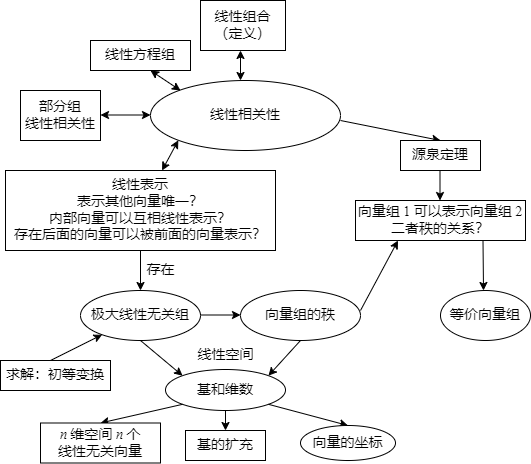
\includegraphics[scale=0.6]{figs/3-1.png}
    \end{figure}

    事实上,与其他内容风格不一样的是,本讲中很大一部分的定理我们都给出了证明,一方面是为了提升阅读体验,防止在初学时就被多个``显然''等词汇困惑,另一方面也是希望读者能够从这些比较规范的证明中得到一些证明的技巧.

    也许读到这里很多读者都会有些迷惑与焦急——为什么我们仿佛在学习很多看起来十分抽象而且似乎没什么实际应用的知识呢?或许我们需要在这里给读者一个``定心丸''. 事实上,我们在上一讲中定义的线性空间运算法则就是从一般向量加法数乘运算法则抽象而来的最为抽象和基本的内容,我们仅仅建立在这一基础上,伴随着线性表示、线性扩张、线性相关等概念的提出,导出了(有限维)线性空间都具有一种统一的本质结构描述——基和维数,由此我们从抽象的运算规则走到了比较具体的结构. 在此基础上,我们基本上将单个线性空间的研究完成,之后我们将会讨论线性空间之间的关系——一方面可以定义线性空间之间的运算,我们将在下一讲详细介绍,另一方面可以建立两个线性空间之间的某种映射,在关于这种映射的讨论中我们会发现线性空间的本质结构是维数,甚至基之间的差异都可以完全被遮蔽(只需通过本讲介绍的坐标即可),然后我们对线性空间的认识便可以从某种比较抽象的结构走向大家熟悉的一定长度的向量,接下来便可以定义更为具象的矩阵. 这一路上我们实际上是从最为抽象的内容逐步定义概念,说明定理,走向具象的内容. 不同于一般线性代数从行列式、矩阵开始,这样的思路一定能让读者对线性代数有更为深刻的认识.

\end{summary}

\begin{exercise}
    \exquote[柯西]{给我五个系数,我将画出一头大象;给我六个系数,大象将会摇动尾巴.}

    \begin{exgroup}
        \item 下列命题是否正确?若正确请证明,否则举出反例.
        \begin{enumerate}
            \item 若 $\alpha_1, \ldots, \alpha_m \ (m > 2)$ 线性相关,则其中每一向量都是其余向量的线性组合;

            \item 若 $\alpha_1, \ldots, \alpha_m$ 线性无关,则其中每一向量不是其余向量的线性组合,这个命题的等价命题应如何叙述?

            \item $\alpha_1, \ldots, \alpha_m \ (m > 2)$ 线性无关的充要条件是任意两个向量都线性无关;

            \item  若 $\alpha_1, \alpha_2$ 线性相关,$ \beta_1, \beta_2$ 线性相关,则 $\alpha_1 + \beta_1, \alpha_2 + \beta_2$ 也线性相关;

            \item 若 $\alpha_1, \ldots, \alpha_n$ 线性无关,则 $\alpha_1 + \alpha_2, \alpha_2 + \alpha_3, \ldots, \alpha_{n-1} + \alpha_n, \alpha_n + \alpha_1$ 也线性无关;

            \item 若 $\alpha_1, \alpha_2, \alpha_3$ 线性相关,则 $\alpha_1 + \alpha_2, \alpha_2 + \alpha_3, \alpha_3 + \alpha_1$ 也线性相关;

            \item 设 $B = \{\alpha_1, \alpha_2, \alpha_3\}$ 是 $ \mathbf{R}^3 $ 的一组基,非零向量 $\alpha_0 \in \mathbf{R}^3$,则 $\{\alpha_0 + \alpha_1, \alpha_0 + \alpha_2, \alpha_0 + \alpha_3\}$ (其中三个向量均是非零向量) 也是 $\mathbf{R}^3$ 的一组基;

            \item  设 $B = \{\alpha_1, \alpha_2\}$ 是 $\mathbf{R}^2$ 的一组基,则 $\{\alpha_1 + \alpha_2, \alpha_1 - \alpha_2\}$ 也是 $\mathbf{R}^2$ 的一组基;

            \item 一个有限维线性空间内只含有有限个子空间;

            \item  若 $W_1, W_2$ 是 $ \mathbf{R}^n $ 的两个子空间,$B_1, B_2$ 分别是 $W_1, W_2$ 的基,则存在 $ \mathbf{R}^n $ 的一组基 $B$,使得 $B \supseteq B_1 \cup B_2$。

        \end{enumerate}
        \begin{answer}
            \begin{enumerate}
                \item 错. 反例:$\alpha_1=(1,0),\alpha_2=(2,0),\alpha_3=(0,1)$,则 $\alpha_1,\alpha_2,\alpha_3$ 线性相关而 $\alpha_3$ 不是 $\alpha_1.\alpha_2$ 的线性组合.

                \item 对. 该命题的等价命题(逆否命题)是:若存在一个向量是其余向量的线性组合,则 $\alpha_1,\ldots,\alpha_m$ 线性相关. 这正是定理 3.1 的内容,因而成立.

                \item 错. 反例:$\alpha_1=(1,0),\alpha_2=(0,1),\alpha_3=(1,1)$,则 $\alpha_1,\alpha_2,\alpha_3$ 两两无关,而三者线性相关. 可证两两无关是向量组无关的必要条件.

                \item 错. 反例:$\alpha_1=(1,0),\alpha_2=(0,0),\beta_1=(0,0),\beta_2=(0,1)$,有 $\alpha_1,\alpha_2$ 相关,$\beta_1,\beta_2$ 相关,而 $\alpha_1+\beta_1$ 与 $\alpha_2+\beta_2$ 线性无关.

                \item 错. 若 $\alpha_1,\ldots,\alpha_n$ 线性无关,有
                    \[\lambda_1\alpha_1+\cdots+\lambda_n\alpha_n\implies\lambda_1=\lambda_2=\cdots=\lambda_n=0,\]
                    判断 $\alpha_1+\alpha_2,\alpha_2+\alpha_3,\ldots,\alpha_n+\alpha_1$ 是否无关. 设
                    \[\lambda_1'(\alpha_1+\alpha_2)+\cdots+\lambda_n'(\alpha_n+\alpha_1)=0,\]
                    则
                    \[(\lambda_n'+\lambda_1')\alpha_1+(\lambda_1'+\lambda_2')\alpha_2+\cdots+(\lambda_{n-1}'+\lambda_{n}')\alpha_n=0,\]
                    则
                    \[\begin{cases} \begin{aligned}
                                \lambda_n'+\lambda_1'       & = 0               \\
                                                            & \vdotswithin{ = } \\
                                \lambda_{n-1}'+\lambda_{n}' & = 0               \\
                            \end{aligned} \end{cases}.\]
                    解该方程可得 $\lambda_n'=(-1)^n\lambda_1'$,因此当 $n$ 为偶数时,上述方程组有非零解,则向量组相关,而当 $n$ 为奇数时,向量组无关. 综上,该命题不成立.

                \item 对. 由定理 3.1,不妨设 $\alpha_3$ 可由 $\alpha_1,\alpha_2$ 线性表示,则 $\alpha_1+\alpha_2,\alpha_2+\alpha_3,\alpha_3+\alpha_1$ 均可由 $\alpha_1,\alpha_2$ 线性表示,再由定理 3.3 可知,$\alpha_1+\alpha_2,\alpha_2+\alpha_3,\alpha_3+\alpha_1$ 线性相关.

                \item 错. 反例:取 $\alpha_0=\alpha_1-\alpha_2-\alpha_3$,则 $\alpha_0+\alpha_1=(\alpha_0+\alpha_2)+(\alpha_0+\alpha_3)$,三者线性相关,不是 $\mathbf{R}^3$ 的基.

                \item 对. 判断 $\alpha_1+\alpha_2$ 与 $\alpha_1-\alpha_2$ 是否无关.
                    \[\lambda_1(\alpha_1+\alpha_2)+\lambda_2(\alpha_1-\alpha_2)=0,\]
                    则有$(\lambda_1+\lambda_2)\alpha_1+(\lambda_1-\lambda_2)\alpha_2=0$,则 $\lambda_1+\lambda_2=0,\lambda_1-\lambda_2=0\implies \lambda_1=\lambda_2=0$,因此线性无关且个数等于维数,是一组基.

                \item 错. 反例:$\mathbf{R}^2$ 中过原点的直线 $L_0$ 是 $\mathbf{R}^2$ 的一个子空间. 显然这样的直线有无数条.

                \item 错. 反例:$\mathbf{R}^3$ 中,子空间 $W_1=\spa(e_1,e_2)$,$W_2=\spa(e_1+e_2,e_3)$,则 $B_1\cup B_2=\{e_1,e_2,e_3,e_1+e_2\}$,显然 $\mathbf{R}^3$ 中的任一组基都不可能包含四个元素.
            \end{enumerate}
        \end{answer}

        \item 证明:如果向量组线性相关,把每个向量去掉$m$个位置一致的分量,得到的缩短组仍线性相关;如果向量组线性无关,把每个向量添加$m$个位置一致的分量,得到的缩短组仍线性无关;
        \begin{answer}
            \begin{enumerate}
                \item 若向量组线性相关,则对应该方程组有无穷多解. 去掉 $m$ 个分量,相当于删去该方程组中的任意 $m$ 行方程,依然有无穷多解. 这是因为对于原方程组的任意一个解,将其带入被削减后的方程组也依然成立. 故线性相关得证.

                \item 若向量组线性无关,对应原方程组仅有唯一解,也就是全零解. 增加 $m$ 个分量相当于增加 $m$ 个方程,依然只有唯一解,因为若出现非零解,代入原方程组对应的方程中不会成立,矛盾. 故线性无关得证.
            \end{enumerate}
        \end{answer}

        \item $a$取何值时,$\beta_1=(1,3,6,2)^\mathrm{T},\beta_2=(2,1,2,-1)^\mathrm{T},\beta_3=(1,-1,a,-2)^\mathrm{T}$线性无关?
        \begin{answer}
            方程组:$x_1\beta_1+x_2\beta_2+x_3\beta_3=0$ 系数矩阵
            \[\begin{pmatrix}
                    1 & 2  & 1  \\
                    3 & 1  & -1 \\
                    6 & 2  & a  \\
                    2 & -1 &
                    -2\end{pmatrix}\rightarrow\begin{pmatrix}
                    1 & 2   & 1   \\
                    0 & -5  & -4  \\
                    0 & -10 & a-6 \\
                    0 & -6  & -4
                \end{pmatrix}\rightarrow\begin{pmatrix}
                    1 & 2  & 1   \\
                    0 & -5 & -4  \\
                    0 & 0  & a+2 \\
                    0 & 0  & 0
                \end{pmatrix},\]
            仅全零解的条件是 $a\neq-2$,此时向量组线性无关.
        \end{answer}

        \item 设$\alpha_1,\alpha_2,\ldots,\alpha_n\in\mathbf{F}^n$. 证明:$\alpha_1,\alpha_2,\ldots,\alpha_n$线性无关的充要条件是$\mathbf{F}^n$中任一向量都可以由它们线性表示.
        \begin{answer}
            \begin{enumerate}
                \item 必要性:$\alpha_1,\ldots,\alpha_n$ 线性无关,对于 $F^n$ 中的任一向量 $\beta$, $\alpha_1,\ldots,\alpha_n,\beta$ 的向量个数大于维数 $n$,则线性相关. 由定理 3.2,$\beta$ 可被 $\alpha_1,\ldots,\alpha_n$ 唯一表示.

                \item 充分性:由于 $F^n$ 中任意向量均可被 $\alpha_1,\ldots,\alpha_n$ 线性表示,并且向量个数等于维数. 则 $\alpha_1,\ldots,\alpha_n$ 是 $F^n$ 的一组基. 则 $\alpha_1,\ldots,\alpha_n$ 线性无关.

                      $^*$ 更详细的证明:对于 $F^n$ 的一组基 $e_1,\ldots,e_n$,其可被 $\alpha_1,\ldots,\alpha_n$ 表示. 若 $\alpha_1,\ldots,\alpha_n$ 线性相关,不妨设 $\alpha_n$ 可被 $\alpha_1,\ldots,\alpha_{n-1}$ 表示,则有 $e_1,\ldots,e_n$ 可被 $\alpha_1,\ldots,\alpha_{n-1}$ 表示. 由于 $e_1,\ldots,e_n$ 线性无关. 根据定理 3.3,$n\leqslant n-1$,矛盾. 因此得证.
            \end{enumerate}
        \end{answer}

        \item 设$S_1=\{\alpha_1,\ldots,\alpha_s\},S_2=\{\beta_1,\ldots,\beta_t\}$是向量空间$V$的两个线性无关的子集,证明:$\alpha_1,\ldots,\alpha_s,\beta_1,\ldots,\beta_t$线性无关$\iff \spa(S_1)\cap \spa(S_2)=\{0\}$.
        \begin{answer}
            \begin{enumerate}
                \item 必要性:对于 $\forall v\in\spa(S_1) \cap \spa(S_2)$ 有 $v=a_1\alpha_1+\cdots+a_s\alpha_s=b_1\beta_1+\cdots+b_t\beta_t$. 由于 $\alpha_1,\ldots,\alpha_s,\beta_1,\ldots,\beta_t$ 线性无关 $\implies a_1=\cdots=a_s=b_1=\cdots=b_t=0$,则 $v=0$,即 $\spa(S_1)\cap\spa(S_2)=\{0\}$.

                \item 充分性:考虑反证法. 如果 $\alpha_1,\ldots,\alpha_s,\beta_1,\ldots,\beta_t$ 线性相关,则存在不全为零的系数使得 $a_1\alpha_1+\cdots+a_s\alpha_s+b_1\beta_1\cdots+b_t\beta_t=0$. 因此存在一个向量 $v=a_1\alpha_1+\cdots+a_s\alpha_s=-(b_1\beta_1\cdots+b_t\beta_t)\neq 0$ 且 $v\in\spa(S_1),v\in\spa(S_2)$. 即存在非零向量 $v$ 属于 $\spa(S_1),v\in\spa(S_2)$,矛盾!则充分性得证.
            \end{enumerate}
        \end{answer}

        \item 完成 \autoref{lem:初等行变换不改变列的线性相关性} 其它两种初等行变换的证明.
        \begin{answer}
            设矩阵为
            \[
                \begin{pmatrix}
                    a_{11} & a_{12} & \cdots & a_{1n} \\
                    a_{21} & a_{22} & \cdots & a_{2n} \\
                    \vdots & \vdots & \ddots & \vdots \\
                    a_{m1} & a_{m2} & \cdots & a_{mn}
                \end{pmatrix},
            \]

            \begin{enumerate}
                \item 对其进行倍乘行变换,即将第 $i$ 行乘以 $c$,那么第 $i$ 行会变为 $c a_{i1}, c a_{i2}, \ldots, c a_{in}$,而其他行不变. 记原先矩阵的列向量为 $S_A = \{\alpha_1,\alpha_2,\ldots,\alpha_n\}$,变换后的矩阵列向量为 $S_B = \{\beta_1,\beta_2,\ldots,\beta_n\}$.

                    先证 $S_A$ 线性相关 $\implies S_B$ 线性相关:若 $S_A$ 线性相关,则存在不全为零的系数 $x_1, x_2, \ldots, x_n$ 使得 $x_1 \alpha_1 + x_2 \alpha_2 + \cdots + x_n \alpha_n = 0$. 由于 $S_B$ 与 $S_A$ 只有第 $i$ 行不同,我们仅需要判断第 $i$ 行中的元素在系数 $x_1, x_2, \ldots, x_n$ 下的线性组合是否为 $0$ 即可. 事实上我们有 $x_1 c a_{i1} + x_2 c a_{i2} + \cdots + x_n c a_{in} = c(x_1 a_{i1} + x_2 a_{i2} + \cdots + x_n a_{in}) = 0$,故 $S_B$ 线性相关.

                    再证 $S_B$ 线性相关 $\implies S_A$ 线性相关:若 $S_B$ 线性相关,由于倍乘行变换保证 $c \neq 0$,故从 $S_B$ 到 $S_A$ 相当于做一次将第 $i$ 行乘以 $\frac{1}{c}$ 的行变换,同理可得 $S_A$ 线性相关.

                    因此,对矩阵做倍乘行变换不改变矩阵的列的线性相关性.

                \item 对其进行对换行变换,即将第 $i$ 行与第 $j$ 行交换,其他行不变. 记原先矩阵的列向量为 $S_A = \{\alpha_1,\alpha_2,\ldots,\alpha_n\}$,变换后的矩阵列向量为 $S_B = \{\beta_1,\beta_2,\ldots,\beta_n\}$.

                    先证 $S_A$ 线性相关 $\implies S_B$ 线性相关:若 $S_A$ 线性相关,则存在不全为零的系数 $x_1, x_2, \ldots, x_n$ 使得 $x_1 \alpha_1 + x_2 \alpha_2 + \cdots + x_n \alpha_n = 0$. 由于 $S_B$ 与 $S_A$ 只有第 $i$ 行与第 $j$ 行不同,我们仅需要判断第 $i$ 行与第 $j$ 行中的元素在系数 $x_1, x_2, \ldots, x_n$ 下的线性组合是否均为 $0$ 即可. 事实上由原先第 $i$($j$)行的元素在 $x_1, x_2, \ldots, x_n$ 下的线性组合为 $0$ 即可得到变换后第 $j$($i$)行的元素的线性组合为 $0$,故 $S_B$ 线性相关.

                    再证 $S_B$ 线性相关 $\implies S_A$ 线性相关:若 $S_B$ 线性相关,从 $S_B$ 到 $S_A$ 相当于再做一次相同的对换行变换,同理有 $S_A$ 线性相关.

                    因此,对矩阵做对换行变换不改变矩阵的列的线性相关性.
            \end{enumerate}
        \end{answer}

        \item 已知$\alpha_1=(1,2,4,3),\alpha_2=(1,-1,-6,6),\alpha_3=(-2,-1,2,-9),\alpha_4=(1,1,-2,7),\beta=(4,2,4,a)$.
        \begin{enumerate}
            \item 求子空间$\spa(\alpha_1,\alpha_2,\alpha_3,\alpha_4)$的维数和一组基;

            \item 求$a$的值使得$\beta\in W$,并求$\beta$在 (1) 所选基下的坐标.
        \end{enumerate}
        \begin{answer}
            \begin{enumerate}
                \item 也就是求 $\alpha_1,\alpha_2,\alpha_3,\alpha_4$ 的极大线性无关组. 利用讲义中所述求法:方程组
                      \[ a_1\alpha_1+\cdots+a_4\alpha_4=0 \]
                      对应系数矩阵 $\begin{pmatrix}
                              1 & 1  & -2 & 1  \\
                              2 & -1 & -1 & 1  \\
                              4 & -6 & 2  & -2 \\
                              3 & 6  & -9 & 7\end{pmatrix}$. 化简为行阶梯型:$\begin{pmatrix}
                              1 & 1  & -2 & 1  \\
                              0 & -3 & 3  & -1 \\
                              0 & 0  & 0  & 3  \\
                              0 & 0  & 0  & 0\end{pmatrix}$,因此 $\alpha_1,\alpha_2,\alpha_3,\alpha_4$ 有非零解,这四个向量线性相关. (其实此处已知矩阵秩为 3,即维数是 3).

                      再选取 $\alpha_1,\alpha_2,\alpha_4$ 来求解方程 $a_1\alpha_1+a_2\alpha_2+a_4\alpha_4=0$:
                      \[\begin{pmatrix}
                              1 & 1  & 1  \\
                              2 & -1 & 1  \\
                              4 & -6 & -2 \\
                              3 & 6  & 7\end{pmatrix}\rightarrow\begin{pmatrix}
                              1 & 1  & 1  \\
                              0 & -3 & -2 \\
                              0 & 0  & 2  \\
                              0 & 0  & 0\end{pmatrix},\]
                      因此该方程组只有全零解,即 $\alpha_1,\alpha_2,\alpha_4$ 是$\alpha_1,\alpha_2,\alpha_3,\alpha_4$的极大线性无关组. 则 $\spa(\alpha_1,\alpha_2,\alpha_4)$ 的维数是 3. 一组基是 $\alpha_1,\alpha_2,\alpha_4$ .

                \item 也就是 $a_1\alpha_1+\cdots+a_4\alpha_4=\beta$有解:增广矩阵 $\begin{pmatrix}
                              1 & 1  & -2 & 1  & 4 \\
                              2 & -1 & -1 & 1  & 2 \\
                              4 & -6 & 2  & -2 & 4 \\
                              3 & 6  & -9 & 7  & a\end{pmatrix}$化为 $\begin{pmatrix}
                              1 & 1  & -2 & 1         & 4   \\
                              0 & -3 & 3  & -1        & -6  \\
                              0 & 0  & 0  & -\frac 83 & 8   \\
                              0 & 0  & 0  & 0         & a-9\end{pmatrix}$,若方程有解,则 $a=9$. 求坐标,取 $x_3=0$ 代入得 $\beta=4\alpha_1+3\alpha_2-3\alpha_4$.
            \end{enumerate}
        \end{answer}

        \item 求解子空间 $V_1 = \{(a,0,b) \mid a,b \in \mathbf{R}\}$ 和 $V_2 = \{(a,2a,b) \mid a,b \in \mathbf{R}\}$ 的基和维数.
        \begin{answer}

        \end{answer}

        \item 证明:$B=\{1,x-a,(x-a)^2\}\enspace(a\neq 0)$是$\mathbf{R}[x]_3$的一组基,并求$\mathbf{R}[x]_3$的自然基$\{1,x,x^2\}$中每个向量关于基$B$的坐标.
        \begin{answer}
            只需证明 $B$ 线性无关即可. $\lambda_1+\lambda_2(x_a)+\lambda_3(x-a)^2$求导,增加方程数得到
            \begin{gather*}
                \lambda_2+2\lambda_3x=0, \\
                2\lambda_3=0,
            \end{gather*}
            则 $\lambda_1=\lambda_2=\lambda_3$,线性无关得证. 又 $B$ 中向量个数等于 $R[x]_3$ 维数. 则 $B$ 是一组基. $1=1 \cdot 1+0 \cdot (x-a)+0\times(x-a)^2$ ,即 $(1,0,0)$;$x=a \cdot 1+1 \cdot (x-a)+0\times(x-a)^2$ ,即 $(a,1,0)$;$x^2=a^2 \cdot 1+2a \cdot (x-a)+1\times(x-a)^2$ ,即 $(a^2,2a,1)$.
        \end{answer}

        \item 已知向量组$A=\{\alpha_1,\alpha_2,\alpha_3\},\enspace B=\{\alpha_1,\alpha_2,\alpha_3,\alpha_4\},\enspace C=\{\alpha_1,\alpha_2,\alpha_3,\alpha_5\}$的秩分别为$r(A)=r(B)=3,\enspace r(C)=4$. 证明:$\{\alpha_1,\alpha_2,\alpha_3,\alpha_5-\alpha_4\}$的秩为4.
        \begin{answer}
            等价于证明 $\alpha_1,\alpha_2,\alpha_3,\alpha_5-\alpha_4$ 线性无关. 即求解
            \begin{equation}
                \lambda_1\alpha_1+\lambda_2\alpha_2+\lambda_3\alpha_3+\lambda_4(\alpha_5-\alpha_4)=0. \tag{*} \label{eq:3:A.10}
            \end{equation}

            由于 $r(A)=r(B)=3$ 可得 $A$ 线性无关. $B$ 线性相关. 由定理 3.2 得 $\alpha_4$ 可由 $\alpha_1,\alpha_2,\alpha_3$ 唯一表示:$\alpha_4=\mu_1\alpha_1+\mu_2\alpha_2+\mu_3\alpha_3$. 则代入 (\ref*{eq:3:A.10}) 式. 有
            \[(\lambda_1-\mu_1\lambda_4)\alpha_1+(\lambda_2-\mu_2\lambda_4)\alpha_2+(\lambda_3-\mu_3\lambda_4)\alpha_3+\lambda_4\alpha_5=0,\]
            因为 $r(C)=4$,$\alpha_1,\alpha_2,\alpha_3,\alpha_5$ 线性无关. 有 $\lambda_4=0,\lambda_1=\mu_1\lambda_4=0,\lambda_2=\mu_2\lambda_4=0,\lambda_3=\mu_3\lambda_4=0$. 故 $\alpha_1,\alpha_2,\alpha_3,\alpha_5-\alpha_4$ 线性无关. 原题得证.
        \end{answer}

        \item 设向量组$\alpha_1,\alpha_2,\ldots,\alpha_s$的秩为$r$. 在其中任取$m$个向量$\alpha_{i1},\alpha_{i2},\ldots,\alpha_{im}$,证明:向量组$\alpha_{i1},\alpha_{i2},\ldots,\alpha_{im}$的秩$\geqslant r+m-s$.
        \begin{answer}
            相当于从 $\alpha_1,\ldots,\alpha_s$ 向量中选取 $s-m$ 个向量丢弃,剩余向量的秩:
            \[r(\alpha_{i1},\ldots,\alpha_{im})\geqslant r-(s-m) =r+m-s.\]
        \end{answer}

        \item 已知$\alpha_1,\alpha_2,\ldots,\alpha_n$线性无关,而$\alpha_1,\alpha_2,\ldots,\alpha_n,\beta,\gamma$线性相关. 证明:要么$\beta,\gamma$可以由$\alpha_1,\alpha_2,\ldots,\alpha_n$线性表示,要么$\alpha_1,\alpha_2,\ldots,\alpha_n,\beta$与$\alpha_1,\alpha_2,\ldots,\alpha_n,\gamma$等价.
        \begin{answer}
            方程:$\lambda_1\alpha_1+\cdots+\lambda_n\alpha_n+\lambda_{n+1}\beta+\lambda_{n+2}\gamma=0$,显然 $\lambda_{n+1},\lambda_{n+2}$ 不全为零. 否则与 $\alpha_1,\ldots,\alpha_n$ 线性无关矛盾.
            \begin{enumerate}
                \item 若 $\lambda_{n+1}=0,\lambda_{n+2}\neq 0$,则 $\gamma$ 可被 $\alpha_1,\ldots,\alpha_n$ 表示. 若 $\lambda_{n+1}\neq0,\lambda_{n+2}=0$, 则 $\beta$ 可被 $\alpha_1,\ldots,\alpha_n$ 表示.

                \item 若 $\lambda_{n+1}\lambda_{n+2}\neq 0$ ,则有
                      \begin{gather*}
                          \beta=-\frac 1{\lambda_{n+1}}(\lambda_1\alpha_1+\cdots+\lambda_n\alpha_n+\lambda_{n+2}\gamma), \\
                          \gamma=-\frac 1{\lambda_{n+2}}(\lambda_1\alpha_1+\cdots+\lambda_n\alpha_n+\lambda_{n+1}\beta).
                      \end{gather*}
                    两组向量可以相互表示. 两者等价. 综上原题得证.
            \end{enumerate}
        \end{answer}
    \end{exgroup}

    \begin{exgroup}
        \item 已知$\alpha_1\neq 0$,则$\alpha_1,\alpha_2,\ldots,\alpha_n$线性相关的充要条件是存在$i\enspace(2 \leqslant i \leqslant n)$使得$\alpha_i$可由$\alpha_1,\alpha_2,\ldots,\alpha_{i-1}$线性表示,且表示法唯一.
        \begin{answer}
            充分性显然成立,下证必要性:由于 $\alpha_1,\ldots,\alpha_n$ 线性相关,则存在 $m$,其能使得 $\alpha_1,\ldots,\alpha_m$ 线性无关的最大下标,有 $1\leqslant m<n$. 因此 $i=m+1$,$\alpha_1,\ldots,\alpha_{i-1}$ 线性无关,$\alpha_1,\ldots,\alpha_i$ 线性相关. 可得 $\alpha_i$ 可被 $\alpha_1,\ldots,\alpha_{i-1}$ 唯一表示.
        \end{answer}

        \item 证明以下两个结论:
        \begin{enumerate}
            \item 设$U$和$W$都是$V$的非零子空间,如果$U\subseteq W$,那么$\dim U \leqslant \dim W$;

            \item 设$U$和$W$都是$V$的非零子空间,$U\subseteq W$,且$\dim U = \dim W$,则$U = W$.
        \end{enumerate}
        \begin{answer}
            \begin{enumerate}
                \item 设 $U$ 的一组基为 $u_1,\ldots,u_m$,$W$ 的一组基为 $w_1,\ldots,w_n$. 由于 $U\subseteq W$,则 $u_1,\ldots,u_m$ 可由 $w_1,\ldots,w_n$ 线性表示,且 $u_1,\ldots,u_m$ 线性无关. 由定理 3.3 的等价命题可得 $m\leqslant n$,则 $m=\dim U\leqslant\dim W=n$ 的得证.

                \item 因为 $\dim U=\dim W$,则 $u_1,\ldots,u_m$ 也是 $W$ 的一组基. 则 $W$ 的任意向量均可由 $u_1,\ldots,u_m$ 表示,可得 $W\subseteq U$,而 $U\subseteq W$,故有 $U=W$ 得证.
            \end{enumerate}
        \end{answer}

        \item 设向量组$\alpha_1,\alpha_2,\ldots,\alpha_n$线性无关. 证明:在向量组$\beta,\alpha_1,\alpha_2,\ldots,\alpha_n$中至多有一个向量$\alpha_i\enspace(1 \leqslant i \leqslant r)$可被其前面的$i$个向量$\beta,\alpha_1,\alpha_2,\ldots,\alpha_{i-1}$线性表示.
        \begin{answer}
            反证法. 若存在两个向量 $\alpha_i,\alpha_j$ 可被前面的向量表示,即
            \begin{gather*}
                \alpha_i=\lambda_0\beta+\lambda_1\alpha_1+\cdots+\lambda_{i-1}\alpha_{i-1}, \\
                \alpha_j=\mu_0\beta+\mu_1\alpha_1+\cdots+\mu_{j-1}\alpha_{j-1}.
            \end{gather*}
            如果 $\lambda_0$ 或者 $\mu_0$ 为 0,则有向量组中的 $\alpha_i$ 或 $\alpha_j$ 可被其他向量线性表示,则该向量组相关,这与条件矛盾. 若 $\lambda_0$ 与 $\mu_0$ 均不为 0,等式可化为
            \begin{gather*}
                \frac 1{\lambda_0}\alpha_i=\beta+\frac{\lambda_1}{\lambda_0}\alpha_1+\cdots+\frac{\lambda_{i-1}}{\lambda_0}\alpha_{i-1}, \\
                \frac 1{\mu_0}\alpha_j=\beta+\frac{\mu_1}{\mu_0}\alpha_1+\cdots+\frac{\mu_{j-1}}{\mu_0}\alpha_{j-1}.
            \end{gather*}
            不妨设 $i>j$. 相减得
            \[\frac 1{\lambda_0}\alpha_i=\left(\frac{\lambda_1}{\lambda_0}-\frac{\mu_1}{\mu_0}\right)\alpha_1+\cdots+\left(\frac{\lambda_i}{\lambda_0}+\frac 1{\mu_0}\right)\alpha_j+\frac{\lambda_{i-1}}{\lambda_0}\alpha_{i-1},\]
            则 $\alpha_i$ 可被其他向量线性表示,因此向量组线性相关,与条件矛盾. 综上,至多有一个向量 $\alpha_i$ 可被前面的相邻线性表示.
        \end{answer}

        \item 证明:$1,e^{\lambda_1\cdot x},e^{\lambda_2\cdot x}$($\lambda_1\neq\lambda_2$且均不为0)线性无关.
        \begin{answer}
            考虑使用求导构造更多方程.
            \[\begin{cases}
                    k_0+k_1\cdot e^{\lambda_1 x}+k_2\cdot e^{\lambda_2 x}=0               \\
                    k_1\lambda_1\cdot e^{\lambda_1 x}+k_2\lambda_2\cdot e^{\lambda_2 x}=0 \\
                    k_1\lambda_1^2\cdot e^{\lambda_1 x}+k_2\lambda_2^2\cdot e^{\lambda_2 x}=0
                \end{cases},\]
          由后两式可知$k_1k_2(\lambda_1-\lambda_0)=0$. 又 $\lambda_1\neq\lambda_2$,故$k_1=k_2=0$,代回第一式得 $k_0=0$,则 $1,e^{\lambda_1x},e^{\lambda_2x}$ 线性无关,得证.
        \end{answer}

        \item 设线性空间$V(\mathbf{F})$中,向量$\beta$是$\alpha_1,\ldots,\alpha_r$的线性组合,但不是$\alpha_1,\ldots,\alpha_{r-1}$的线性组合. 证明:$\spa(\alpha_1,\ldots,\alpha_{r-1},\alpha_r)=\spa(\alpha_1,\ldots,\alpha_{r-1},\beta)$.
        \begin{answer}
            只需证明 $\alpha_r$ 可以被 $\alpha_1,\ldots,\alpha_{r-1},\beta$ 表示即可. 由于 $\beta$ 是 $\alpha_1,\ldots,\alpha_{r-1}$ 的线性组合,若 $\lambda_r=0$,则 $\beta$ 是 $\alpha_1,\ldots,\alpha_{r-1}$ 的线性组合. 这与条件矛盾. 因此 $\alpha_r=-\vspace{1ex}\dfrac 1{\lambda_r}(\lambda_1\alpha_1+\cdots+\lambda_{r-1}\alpha_{r-1}-\beta)$,则这两组向量等价. $\spa(\alpha_1,\ldots,\alpha_{r-1},\alpha_r)=\spa(\alpha_1,\ldots,\alpha_{r-1},\beta)$ 得证.
        \end{answer}

        \item \label{item:3:正实数线性空间}
        设$\mathbf{R}^+$是所有正实数组成的集合,加法和数乘定义如下:
        \[ \forall a,b \in \mathbf{R}_+,\enspace k\in \mathbf{R}\colon\enspace a\oplus b = ab,\enspace k\odot a = a^k \]
        则 $\mathbf{R}^+$关于这一加法和数乘构成一个实线性空间. 求$\mathbf{R}^+$的一组基.
        \begin{answer}
            分析该实线性空间,可以看出加法单位元为 1,数乘单位元为 1. 我们给出一组基:$e$,其中 $e$ 为自然对数的底数. 当然, 2,3 或者 10 都可以作为一组基. 接下来我们验证 $e$ 是 $\mathbf{R}^+$ 的基:$\forall a\in \mathbf{R}^+,\exists k=\ln a\in\mathbf{R}$,满足 $k\odot e=e^k=a$,则 $\spa(e)=\mathbf{R}^+$ 成立. 由于该向量组只有一个元素,且并非设该空间的零元 1,则 $e$ 是线性无关的. 得证.
        \end{answer}
    \end{exgroup}

    \begin{exgroup}
        \item 已知$m$个向量$\alpha_1,\alpha_2,\ldots,\alpha_m$线性相关,但其中任意$m-1$个都线性无关,证明:
        \begin{enumerate}
            \item 若$k_1\alpha_1+\cdots+k_m\alpha_m=0$,则$k_1,\ldots,k_m$全为0或全不为0;

            \item 若以下等式成立
                  \begin{align*}
                      k_1\alpha_1+\cdots+k_m\alpha_m & =0 \\
                      l_1\alpha_1+\cdots+l_m\alpha_m & =0
                  \end{align*}
                  其中$l_1\neq 0$,证明:$\dfrac{k_1}{l_1}=\cdots=\dfrac{k_m}{l_m}$.
        \end{enumerate}
        \begin{answer}
            \begin{enumerate}
                \item 若 不全为 0. 不妨设设至少有 $k_i=0$,则有 $k_1\alpha_1+\cdots+k_{i-1}\alpha_{i-1}+k_{i+1}\alpha_{i+1}+\cdots+k_m\alpha_m=0$,并且系数不全为 0. 因此 $\alpha_1,\ldots,\alpha_{i-1},\alpha_{i+1},\ldots,\alpha_m$ 这 $m-1$ 个向量相关,与题设矛盾. 则原题得证.

                \item $l_1\neq 0$,则 $l_2,\ldots,l_m$ 均不为 0.
                      \begin{enumerate}
                          \item 若 $k_1=\cdots=k_m=0$. 原式显然成立.

                          \item 若 $k_1,\ldots,k_m$ 不全为 0. 则
                                \begin{gather*}
                                    l_1(k_1\alpha_1+\cdots+k_m\alpha_m)=0, \\
                                    k_1(l_1\alpha_1+\cdots+l_m\alpha_m)=0.
                                \end{gather*}
                                两式相减,得
                                \[(k_2l_1-k_1l_2)\alpha_2+\cdots+(k_ml_1-k_1l_m)\alpha_m=0,\]
                                因为 $\alpha_2,\ldots,\alpha_m$ 线性无关. 则以上系数均为 0. 故$\dfrac {k_2}{l_2}=\dfrac {k_1}{l_1},\ldots,\dfrac {k_m}{l_m}=\dfrac {k_1}{l_1}$. 得证.
                      \end{enumerate}
            \end{enumerate}
        \end{answer}

        \item (替换定理)设$\alpha_1,\alpha_2,\ldots,\alpha_r$线性无关,且可以被$\beta_1,\beta_2,\ldots,\beta_n$线性表示,则可以将$\beta_1,\beta_2,\ldots,\beta_n$中的$r$个向量替换成$\alpha_1,\alpha_2,\ldots,\alpha_r$后得到与$\beta_1,\beta_2,\ldots,\beta_n$等价的新向量组(注:可以使用数学归纳法证明).
        \begin{answer}
            利用递推法:当 $r=1$ 时,由于 $\alpha_1$ 线性无关,可得 $\alpha_1\neq 0$. 设 $\alpha_1=\lambda_1\beta_1+\cdots+\lambda_n\beta_n$,则至少存在一个 $\lambda_i\neq 0$,不妨设 $\lambda_1\neq 0$,因此有 $\beta_1=-\vspace{1ex}\dfrac 1{\lambda_1}(-\alpha_1+\lambda_2\beta_2+\cdots+\lambda_n\beta_n)$,故 $\beta_1,\ldots,\beta_n$ 与 $\alpha_1,\beta_2,\ldots,\beta_n$ 等价.

            当 $r=2$ 时,由于 $\alpha_1,\alpha_2$ 无关. 有 $\alpha_1\alpha_2\neq 0$. 根据 $r=1$ 的情况,不妨设 $\beta_1,\ldots,\beta_n$ 与 $\alpha_1,\beta_2,\ldots,\beta_n$ 等价. 因此 $\alpha_2$ 可由 $\alpha_1,\beta_2,\ldots,\beta_n$ 表出:
            \[\alpha_2=\mu_1\alpha_1+\mu_2\beta_2+\cdots+\mu_n\beta_n.\]
            由于 $\alpha_1,\alpha_2$ 无关,故 $\mu_2,\ldots,\mu_n$ 至少有一个非零的数. 不妨设 $\mu_2\neq 0$,同上可得$\alpha_1,\alpha_2,\beta_3,\ldots,\beta_n$ 就与 $\alpha_1,\beta_2,\ldots,\beta_n$ 等价,也与$\beta_1,\beta_2,\ldots,\beta_n$ 等价. 综上,通过递推可知,对正整数 $r$,上述结论依然成立.
        \end{answer}

        \item 设线性空间$V=\mathbf{F}^n$. 证明:
        \begin{enumerate}
            \item 存在$V$的子空间$W$,使得$W$的任一非零向量的分量均不为0;

            \item 若$V$的子空间$W$的任一非零向量的分量均不为0,则$\dim W=1$;

            \item 若$V$的子空间$W$的任一非零向量的零分量个数均不超过$r$,则$\dim W \leqslant r+1$.
        \end{enumerate}
        \begin{answer}
            \begin{enumerate}
                \item $\alpha=(1,1,\ldots,1)^{\mathrm{T}}, W=\spa(\alpha)$,显然 $W$ 是满足条件的一维子空间.

                \item 考虑反证法:若 $\dim W>1$,则 $W$ 中存在线性无关的两向量. 由条件,
                      \[a_1,\ldots,a_n,b_1,\ldots,b_n\neq 0,\]
                      可设 $a_1=kb_1,k\in F$,因此 $\alpha-k\beta=(0,a_2-kb-2,\ldots,a_n-kb_n)^{\mathrm{T}}\in W$. 且由于 $\alpha,\beta$ 无关,$\alpha-k\beta\neq 0$ 但存在分量为 0,这与条件矛盾. 故 $\dim W=1$.

                \item 考虑反证法:若 $\dim W>r+1$,则存在 $r+2$ 个线性无关的向量,设为
                      \begin{align*}
                          \alpha_1     & = (a_{11},a_{12},\ldots,a_{1(r+1)},\ldots,a_{1n})^{\mathrm{T}},                 \\
                                       & \vdotswithin{ = }                                                              \\
                          \alpha_{r+2} & = (a_{(r+2)1},a_{(r+2)2},\ldots,a_{(r+2)(r+1)},\ldots,a_{(r+2)n})^{\mathrm{T}}.
                      \end{align*}
                      取这些向量的前 $r+1$ 个分量组成新的向量组:
                      \begin{align*}
                          \beta_1     & = (a_{11},a_{12},\ldots,a_{1(r+1)})^{\mathrm{T}},             \\
                                      & \vdotswithin{ = }                                            \\
                          \beta_{r+2} & = (a_{(r+2)1},a_{(r+2)2},\ldots,a_{(r+2)(r+1)})^{\mathrm{T}}.
                      \end{align*}
                      由于 $\beta_1,\ldots,\beta_{r+2}$ 是 $r+2$ 个 $r+1$ 维向量,其必然线性相关,则存在不全为 0 的系数 $\lambda_1,\ldots,\lambda_{r+2}$,$\lambda_1\beta_1+\cdots+\lambda_{r+2}\beta_{r+2}=0$.  由于 $\alpha_1,\ldots,\alpha_{r+2}$ 线性无关知:$\lambda_1\alpha_1+\cdots+\lambda_{r+2}\alpha_{r+2}\neq 0$,且其属于 $W$. 但其前 $r+1$ 个分量均为 0,这与条件矛盾. 故 $\dim W\leqslant r+1$ 得证.
            \end{enumerate}
        \end{answer}

        \item 设 $\mathbf{Q}(\sqrt[3]{2}) = \{a+b\sqrt[3]{2}+c\sqrt[3]{4}\mid a,b,c\in\mathbf{Q}\}$,证明 $\mathbf{Q}(\sqrt[3]{2})$ 是 $\mathbf{Q}$ 上的线性空间并求其维数.
        \begin{answer}
            先证明 $\mathbf{Q}(\sqrt[3]{2})$ 是 $\mathbf{Q}$ 上的线性空间:

            $\mathbf{Q}(\sqrt[3]{2})$ 对通常的加法构成交换群以及其封闭性是显然的,在此不再赘述,下阐述数乘性质:
            \begin{enumerate}
                \item $\forall v = a+b\sqrt[3]{2}+c\sqrt[3]{4} \in \mathbf{Q}(\sqrt[3]{2}), \enspace 1 (a+b\sqrt[3]{2}+c\sqrt[3]{4}) = a+b\sqrt[3]{2}+c\sqrt[3]{4}$;

                \item $\forall v = a+b\sqrt[3]{2}+c\sqrt[3]{4} \in \mathbf{Q}(\sqrt[3]{2}), \forall \lambda, \mu \in \mathbf{Q}, \enspace \lambda(\mu v) = (\lambda \mu) v$;

                \item $\forall v = a+b\sqrt[3]{2}+c\sqrt[3]{4} \in \mathbf{Q}(\sqrt[3]{2}), \forall \lambda, \mu \in \mathbf{Q}, \enspace (\lambda + \mu) v = (\lambda + \mu)a + (\lambda + \mu) b\sqrt[3]{2} + (\lambda + \mu) c\sqrt[3]{4} = \lambda(a+b\sqrt[3]{2}+c\sqrt[3]{4}) + \mu(a+b\sqrt[3]{2}+c\sqrt[3]{4}) = \lambda v + \mu v$;

                \item $\forall v = a_1 + b_1\sqrt[3]{2} + c_1\sqrt[3]{4}, u = a_2 + b_2\sqrt[3]{2} + c_2\sqrt[3]{4} \in \mathbf{Q}(\sqrt[3]{2}), \forall \lambda \in \mathbf{Q}, \enspace \lambda(v+u) = \lambda (a_1 + a_2) + \lambda (b_1 + b_2)\sqrt[3]{2} + \lambda (c_1 + c_2)\sqrt[3]{4} = \lambda (a_1 + b_1\sqrt[3]{2} + c_1\sqrt[3]{4}) + \lambda (a_2 + b_2\sqrt[3]{2} + c_2\sqrt[3]{4}) = \lambda v + \lambda u$;

                \item (封闭性)$\forall v = a+b\sqrt[3]{2}+c\sqrt[3]{4} \in \mathbf{Q}(\sqrt[3]{2}), \forall \lambda \in \mathbf{Q}, \enspace \lambda v = \lambda a + \lambda b\sqrt[3]{2} + \lambda c\sqrt[3]{4} \in \mathbf{Q}(\sqrt[3]{2})$.
            \end{enumerate}
            故 $\mathbf{Q}(\sqrt[3]{2})$ 是 $\mathbf{Q}$ 上的线性空间.

            下求 $\mathbf{Q}(\sqrt[3]{2})$ 的维数. 考虑找 $\mathbf{Q}(\sqrt[3]{2})$ 的一组基,我们给出 $\{1, \sqrt[3]{2}, \sqrt[3]{4}\}$,下证其为 $\mathbf{Q}(\sqrt[3]{2})$ 的一组基:

            \begin{enumerate}
                \item (线性无关)令 $k_1 + k_2 \sqrt[3]{2} + k_3 \sqrt[3]{4} = 0$,其中 $k_1, k_2, k_3 \in \mathbf{Q}$,由于左边只有第一项为有理数,故有 $k_1 = 0$,进而有 $\sqrt[3]{2} (k_2 + k_3 \sqrt[3]{2}) = 0$,又可得到 $k_2 = 0$,并且 $k_3 = 0$. 故 $\{1, \sqrt[3]{2}, \sqrt[3]{4}\}$ 线性无关.

                \item (张成空间)由 $\mathbf{Q}(\sqrt[3]{2})$ 的定义易得.
            \end{enumerate}
            综上,$\mathbf{Q}(\sqrt[3]{2})$ 是 $\mathbf{Q}$ 上的线性空间,且 $\dim \mathbf{Q}(\sqrt[3]{2}) = 3$.

        \end{answer}

        \item 设$\mathbf{K} \subseteq \mathbf{F} \subseteq \mathbf{E}$是三个数域,已知$\mathbf{F}$作为$\mathbf{K}$上的线性空间是$n$维的,$\mathbf{E}$作为$\mathbf{F}$上的线性空间是$m$维的,证明:$\mathbf{E}$作为$\mathbf{K}$上的线性空间是$mn$维的.
        \begin{answer}
            取 $\mathbf{F}(\mathbf{K})$ 的一组基 $f_1, f_2, \ldots, f_n$,$\mathbf{E}(\mathbf{F})$ 的一组基 $e_1, e_2, \ldots, e_m$,下证向量组 $B = \{f_1 e_1, f_2 e_1, \ldots, f_n e_1, f_1 e_2, f_2 e_2, \ldots, f_n e_2, \ldots, f_1 e_m, f_2 e_m, \ldots, f_n e_m\}$ 是 $\mathbf{E}(\mathbf{K})$ 的一组基:

            \begin{enumerate}
                \item (线性无关)令 $k_{11} f_1 e_1 + k_{12} f_2 e_1 + \cdots + k_{1n} f_n e_1 + k_{21} f_1 e_2 + k_{22} f_2 e_2 + \cdots + k_{2n} f_n e_2 + \cdots + k_{m1} f_1 e_m + k_{m2} f_2 e_m + \cdots + k_{mn} f_n e_m = 0$,其中 $k_{ij} \in \mathbf{K}$,则
                    \[
                        \sum_{i=1}^m \left(\sum_{j=1}^n k_{ij} f_j \right) e_i = 0.
                    \]
                    由于 $e_1, e_2, \ldots, e_n$ 是 $\mathbf{E}(\mathbf{F})$ 的一组基 $e_1, e_2, \ldots, e_m$,我们有
                    \[
                        \sum_{j=1}^n k_{ij} f_j = 0, \enspace \forall i = 1, 2, \ldots, m.
                    \]
                    而 $f_1, f_2, \ldots, f_n$ 又是 $\mathbf{F}(\mathbf{K})$ 的一组基,故 $k_{ij} = 0$,即向量组 $B$ 线性无关.

                \item (张成空间)$\forall e = \mu_1 e_1 + \mu_2 e_2 + \cdots + \mu_m e_m \in \mathbf{E} \enspace (\mu_1, \mu_2, \ldots, \mu_m \in \mathbf{F})$,由于 $\mu_i \in \mathbf{F}$,故存在 $k_{ij} \in \mathbf{K}$ 使得 $\mu_i = k_{i1} f_1 + k_{i2} f_2 + \cdots + k_{in} f_n$,于是
                    \[
                        e = \sum_{i=1}^m \left(\sum_{j=1}^n k_{ij} f_j \right) e_i
                          = \sum_{i=1}^m \sum_{j=1}^n k_{ij} f_j e_i.
                    \]
                    故 $e \in \spa B$.
            \end{enumerate}
            综上,$B$ 是 $\mathbf{E}(\mathbf{K})$ 的一组基,故 $\dim \mathbf{E}(\mathbf{K}) = mn$.
        \end{answer}

        \item 延续上一讲对于 $\mathbf{F_4}(\mathbf{Z}_2)$ 的讨论,尝试求 $\mathbf{F_4}$ 在 $\mathbf{Z}_2$ 上的一组基及其维数,以及其中每个元素的坐标表示.
        \begin{answer}

        \end{answer}
    \end{exgroup}
\end{exercise}
